\documentclass[
    iai, % Saisir le nom de l'institut rattaché
    eai, % Saisir le nom de l'orientation
    %confidential, % Décommentez si le travail est confidentiel
]{heig-tb}

\usepackage[nooldvoltagedirection,european,americaninductors]{circuitikz}

\signature{signature.svg}

\makenomenclature
\makenoidxglossaries
\makeindex

\addbibresource{bibliography.bib}

\input{nomenclature}
\input{acronyms}
\input{glossary}
% Auteur du document (étudiant-e) en projet de Bachelor
\author{Tristan Lieberherr}

% Activer l'option pour l'accord du féminin dans le texte
\genre{male}

% Titre de votre travail de Bachelor
\title{Gestion centralisée des demandes de travaux pour le FabLab HEIG-VD}

% Le sous titre est optionnel
\subtitle{Travail de Bachelor}

% Nom du professeur responsable
\teacher {Prof. Y. Chevallier (HEIG-VD)}

% Mettre à jour avec la date de rendu du travail
\date{\today}

% Numéro de TB
\thesis{7212}



%\surroundwithmdframed{minted}
\graphicspath{{assets/figures/}}

%% Début du document
\begin{document}
\selectlanguage{french}
\maketitle
\frontmatter
\clearemptydoublepage

%% Requis par les dispositions générales des travaux de Bachelor
\preamble
\authentification

%% Résumé / Version abbrégée
\begin{abstract}
  % Francais
Le but de ce travail de Bachelor est de mettre en place une plateforme web dédiée à la demande de travaux pour le FabLab.
Actuellement, la procédure est mal définie : les échanges se font manuellement par email et il n'y a pas de suivi des commandes traçable, ce qui peut impliquer des confusions, des retards de fabrication, etc.

Avec cette nouvelle plateforme, la procédure sera claire et automatisée.
Les techniciens et les clients pourront communiquer entre eux en temps réel et auront la possibilité d'avoir une vue de l'avancement du projet.
Un système de notification personnalisable sera disponible pour informer rapidement les utilisateurs concernant l'avancement de leurs demandes.
De plus, le système sera réactif : il sera accessible et ergonomique autant sur un PC que sur un smartphone.

L'interface utilisera l'authentification via Switch AAI, le même service qui est utilisé pour se connecter à son compte GAPS ou Cyberlearn, ce qui signifie que tous les étudiants y auront directement accès, sans avoir à se créer un compte.

\asterism

% English
The goal of this Bachelor's thesis is to create a web platform for submitting job requests to the FabLab.
Currently, the procedure is not well defined : communication is manually done by email and there is no way to monitor the job's progress, wich may cause confusions, production delays, etc.

With this new platform, the procedure will be clear and automated.
Both technicians and clients will be able to communicate in real time and have access to an overview of the job's progress.
A customizable notification system will be available to quickly inform the users about their job's progress.
Furthermore, the system will be reactive : it will be available and adaptive for both PC and smartphone screens.

The interface will use Switch AAI's authentication, the same service that is used to connect to GAPS or Cyberlearn, wich means that all students will have direct access, without the need to create an account.
\end{abstract}

%% Sommaire et tables
\clearemptydoublepage
{
  \tableofcontents
  \let\cleardoublepage\clearpage
  \listoffigures
  \let\cleardoublepage\clearpage
  \listoftables
  \let\cleardoublepage\clearpage
  \listoflistings
}

\printnomenclature
\clearemptydoublepage
\pagenumbering{arabic}

\usemintedstyle{xcode}

%% Contenu
\mainmatter
\chapter{Introduction}
\section{Contexte}
En l'état actuel, il n'y a pas de système automatisé pour déposer des demandes de travaux au FabLab. Il faut s'adresser à un technicien et discuter avec pour pouvoir lui soumettre son projet, et attendre qu'il ait fini avant d'aller récupérer le résultat. Pendant le temps où le technicien est à l'oeuvre, le client n'a aucune idée de l'état d'avancement de sa demande. En cas de souci, le technicien doit recontacter le client, lui demander des clarifications ou des fichiers, avant de pouvoir continuer.

D'après la description de la procédure actuelle, il est possible de mettre en évidence les défauts :

\begin{enumerate}
  \item Aucun suivi des travaux pour le client
  \item Échanges éparpillés : email, vocal
  \item Risque de désorganisation
  \item Manque de clarté quant à la procédure
\end{enumerate}

\section{Cas d'utilisation}
Pour répondre aux problèmes mis en évidence, j'ai imaginé la nouvelle procédure de demandes de travaux. Dans cette procédure, il y a deux acteurs :

\begin{itemize}
  \item Le client : personne qui dépose la demande
  \item Le technicien : personne qui s'occupe de réaliser le travail
\end{itemize}

Cas de figure :

Le client veut réaliser une pièce fraisée pour son projet multidisciplinaire. Il se connecte sur l'interface web via le login Switch AAI, comme il en a l'habitude avec les autres services proposés par l'école. Arrivé sur la page, il peut consulter la liste des travaux réalisables, avant de remplir le formulaire. Il indique le type de travail parmi ceux disponibles, y dépose éventuellement les fichiers nécessaires et envoie la demande. Il peut voir que sa demande figure désormais dans sa liste de demandes.

Du côté du technicien, il a accès à la liste de tous les travaux déposés. Quand il voit la nouvelle demande, il se l'attribue et peut désormais voir toutes les informations du travail : type, fichiers, commentaire et messages. Lorsqu'il se met au travail, il fait changer l'état de la demande, pour que le client puisse consulter l'avancement.
Malheureusement, il manque un fichier crucial pour la réalisation et il se retrouve bloqué. Il change l'état de la demande, et envoie un message instantané au client, lui demandant d'ajouter le fichier manquant.

Quand le client est notifié par mail de ce changement d'état, il se connecte et voit qu'il a reçu un nouveau message lui demandant d'ajouter le fichier. C'est donc ce qu'il fait : il ajoute le fichier et remercie le technicien de l'avoir prévenu.

Le technicien, notifié par l'ajout du fichier, télécharge ce dernier et peut se remettre au travail. Lorsque le travail est terminé, il l'indique pour que le client puisse venir chercher la pièce.

Le client, une fois la pièce récupérée et le technicien remercié, évalue la qualité du travail avant de disposer de la demande désormais accomplie.

\figi{BPMN.xml}{14cm}{Diagramme BPMN du cas d'utilisation}

Bien sûr, les échanges seront disponibles en toutes circonstances, dès lors que le travail a été assigné à un technicien. Les acteurs pourront en tout temps s'échanger des messages instantanés et des fichiers.

\newpage
\section{Cahier des charges}
Le cahier des charges a été établi dès le début du projet et n'a pas eu besoin d'être mis à jour par la suite.
Dans ce cahier des charges, je me suis engagé à réaliser les tâches suivantes :

\begin{enumerate}
  \item Réaliser une interface web pour la gestion des demandes de travaux, qui comporte au moins les fonctionnalités suivantes :
        \begin{itemize}
          \item Liste des prestations offertes
          \item Faire une demande de travail pour une des prestations offertes
          \item Suivi en temps réel de l'état d'avancement de la demande
          \item Échange de fichiers et de messages avec le technicien
          \item Personnaliser les notifications par email
          \item Les techniciens ont accès aux demandes de travaux déposées par les clients
          \item Les techniciens peuvent faire évoluer l'état d'avancement des demandes
        \end{itemize}
  \item Assurer une interface responsive et réactive (depuis smartphone)
  \item Architecturer la base de données
  \item Coder le backend : ORM, gestion des demandes, notifications
  \item Déployer l'interface sur une VM de l'école
  \item Réaliser les tests de fonctionnement
\end{enumerate}
\bigskip
Ce cahier des charges garantit que le système final de ce projet sera opérationnel.

\newpage
\section{Analyse des besoins et fonctions}
En fonction du cahier des charges et du cas d'utilisation, j'ai pu relever les besoins des utilisateurs.
Je les ai regroupés en deux tableaux, pour les clients et les techniciens.

\begin{table}[h]
  \begin{center}
    \caption{Besoins des clients}
    \begin{tabularx}{\textwidth}{cXc}
      No.  & Besoin                                                                                                         \\ \toprule
      N1.1 & Être capable de déposer des demandes de travaux                                                                \\ \midrule
      N1.2 & Être capable de consulter les demandes déposées et leur état d'avancement, fichiers joints et messages envoyés \\ \midrule
      N1.3 & Besoin d'être averti en étant hors-ligne d'évènements liés aux demandes                                        \\ \midrule
      N1.4 & Nécessité de pouvoir communiquer efficacement avec le technicien, d'échanger des messages et des fichiers avec \\ \midrule
      N1.5 & Pouvoir accéder et interagir avec l'interface depuis un PC ou un smartphone                                    \\ \midrule
      N1.6 & Besoin de récupérer et d'évaluer le travail accompli                                                           \\ \midrule
    \end{tabularx}
  \end{center}
\end{table}

\begin{table}[h]
  \begin{center}
    \caption{Besoins des techniciens}
    \begin{tabularx}{\textwidth}{cXc}
      No.  & Besoin                                                                                                          \\ \toprule
      N2.1 & Avoir la possibilité de consulter les demandes non-assignées et de se les assigner                              \\ \midrule
      N2.2 & Être capable de consulter les demandes assignées et leur état d'avancement, fichiers joints et messages envoyés \\ \midrule
      N2.3 & Être capable de mettre à jour l'état d'avancement des commandes assignées                                       \\ \midrule
      N2.4 & Besoin d'être averti en étant hors-ligne d'évènements liés aux demandes                                         \\ \midrule
      N2.5 & Nécessité de pouvoir communiquer efficacement avec le client, d'échanger des messages et des fichiers avec      \\ \midrule
      N2.6 & Pouvoir accéder et interagir avec l'interface depuis un PC ou un smartphone                                     \\ \midrule
    \end{tabularx}
  \end{center}
\end{table}

\newpage
Afin de répondre à ces besoins identifiés, j'ai pu établir le tableau des fonctions, qui liste les fonctionnalités auxquelles les utilisateurs auront accès.

\begin{table}[h]
  \begin{center}
    \caption{Fonctions du système}
    \begin{tabularx}{\textwidth}[t]{p{0.5cm}Xp{1cm}}
      No. & Fonction                                                                                                                                                                                   & Besoin No.         \\ \toprule
      F1  & Créer une nouvelle demande de travail via un formulaire adaptatif en fonction du type de travail, avec possibilité de joindre des fichiers et un commentaire à l'intention des techniciens & N1.1               \\ \midrule
      F2  & Visualiser une liste des demandes déposées ou assignées, contenant pour chaque demande toutes les informations associées                                                                   & N1.2 \newline N2.2 \\ \midrule
      F3  & Visualiser une liste de toutes les demandes non-assignées, contenant pour chaque demande les informations du formulaire                                                                    & N2.1               \\ \midrule
      F4  & Possibilité de s'assigner des demandes non-assignées                                                                                                                                       & N2.1               \\ \midrule
      F5  & Échanger des messages instantanés depuis un salon de discussion lié à une demande                                                                                                          & N1.4 \newline N2.5 \\ \midrule
      F6  & Ajouter des fichiers à une demande                                                                                                                                                         & N1.4 \newline N2.5 \\ \midrule
      F7  & Possibilité de personnaliser les notifications par mail en fonction des évènements liés à une demande                                                                                      & N1.3 \newline N2.4 \\ \midrule
      F8  & Modifier l'état des demandes                                                                                                                                                               & N2.3               \\ \midrule
      F9  & Adaptation automatique de l'interface graphique au type et à la taille de l'écran de l'appareil utilisé                                                                                    & N1.5 \newline N2.6 \\ \midrule
      F10 & Suppression d'une demande terminée                                                                                                                                                         & N1.6               \\ \midrule
      F11 & Évaluation du travail accompli                                                                                                                                                             & N1.6               \\ \midrule
    \end{tabularx}
  \end{center}
\end{table}

\newpage
\section{Choix technologiques}
Le monde du développement web est un univers totalement nouveau pour moi.
Au cours de ma formation, j'ai acquis des compétences très basiques en HTML, PHP et JavaScript.
Je n'ai par conséquent jamais utilisé de framework auparavant.
Après avoir exploré le net et consulté mon mentor, j'ai découvert qu'il existait une multitude de frameworks.
J'ai ensuite sommairement rempli un tableau qui regroupe certains des frameworks populaires afin d'établir un comparatif, pour mettre en évidence les avantages et les inconvénients de chacun.

Étant donné la prédisposition pour les frameworks Laravel et Vue, comme expliqué plus loin, j'ai limité le nombre de frameworks dans les tableaux.
J'ai choisi parmi les plus populaires, car en général, si un outil est populaire, il sera facile de trouver des réponses et des solutions sur internet.
En vérifiant sur StackOverflow, j'ai trouvé à \href{https://insights.stackoverflow.com/trends}{cette adresse} un outil qui génère des graphiques montrant la tendance de certains sujets.

\begin{table}[h]
  \begin{center}
    \caption{Comparaison des bases de données}
    \begin{tabularx}{\textwidth}[t]{m{0.5cm}Xp{4cm}p{4cm}}
      No.                            & Technologie     & Avantages & Inconvénients \\ \toprule
      1                              & MySQL           & 
      \textbf{+} Relationnelle \newline
      \textbf{+} Très populaire
                                     & 
      \textbf{--} Convient mal pour stocker énormément de données                  \\ \midrule
      2                              & MongoDB         & 
      \textbf{+} Performante         & 
      \textbf{--} Non relationnelle                                                \\ \midrule
      3                              & PostgreSQL      & 
      \textbf{+} Riche en fonctionnalités \newline
      \textbf{+} Relationnelle/objet & 
      \textbf{--} Plus complexe que MySQL                                          \\ \midrule
      4                              & Oracle Database & 
      \textbf{+} Relationnelle       & 
      \textbf{--} Payante                                                          \\ \midrule
    \end{tabularx}
  \end{center}
\end{table}

\figi{stackoverflow_trends_DB.svg}{13cm}{StackOverflow, questions par mois, database}
%% https://insights.stackoverflow.com/trends?tags=mysql%2Cmongodb%2Cpostgresql%2Coracle
\newpage

Au final, j'ai choisi MySQL comme base de données.

Pourquoi MySQL ? Car c'est ce qui semble être LA base de données par défaut. Elle est gratuite, populaire, je m'en suis déjà servi et à défaut d'avoir besoin de spécifications particulières en terme de performances, elle convient très bien à n'importe quel projet.
Il fallait aussi que ce soit une base relationnelle, c'est à dire avec des tables de modèles définis.

\begin{table}[h]
  \begin{center}
    \caption{Comparaison des frameworks backend}
    \begin{tabularx}{\textwidth}[t]{m{0.5cm}Xp{4.7cm}p{4.7cm}}
      No. & Technologie & Avantages & Inconvénients \\ \toprule
      1   & Laravel     & 
      \textbf{+} Simple \newline
      \textbf{+} Professeur expérimenté
          & 
      \textbf{--} Convient moins bien aux gros projets
      \\ \midrule
      2   & Django      & 
      \textbf{+} Développement rapide
          & 
      \textbf{--} Python
      \\ \midrule
      3   & Express     & 
      \textbf{+} JavaScript
          & 
      \textbf{--} Nature asynchrone
      \\ \midrule
      4   & Rails       & 
      \textbf{+} Simple
          & 
      \textbf{--} Ruby
      \\ \midrule
    \end{tabularx}
  \end{center}
\end{table}

\figi{stackoverflow_trends_backend.svg}{13cm}{StackOverflow, questions par mois, backend}
%% https://insights.stackoverflow.com/trends?tags=laravel%2Cdjango%2Cexpress%2Cruby-on-rails

Au final, j'ai choisi Laravel comme framework backend.

Pourquoi Laravel ? Car c'est un framework très simple pour les débutants comme moi, et que mon professeur responsable sait déjà s'en servir.
En cas de problèmes, il saura m'aider et m'orienter, ce qui selon moi justifie pleinement l'utilisation de ce framework en particulier.
\newpage

\begin{table}[h]
  \begin{center}
    \caption{Comparaison des frameworks frontend}
    \begin{tabularx}{\textwidth}[t]{m{0.5cm}Xp{4.7cm}p{4.7cm}}
      No. & Technologie & Avantages & Inconvénients \\ \toprule
      1   & Angular     & 
      \textbf{+} Très complet
          & 
      \textbf{--} Complexe
      \\ \midrule
      2   & React       & 
      \textbf{+} Simple
          & 
      \textbf{--} JavaScript XML
      \\ \midrule
      3   & Vue         & 
      \textbf{+} Simple \newline
      \textbf{+} PIAF utilise Vue
          & 
      \textbf{--} Trop flexible
      \\ \midrule
    \end{tabularx}
  \end{center}
\end{table}

\figi{stackoverflow_trends_frontend.svg}{13cm}{StackOverflow, questions par mois, frontend}
%% https://insights.stackoverflow.com/trends?tags=reactjs%2Cvue.js%2Cangular%2Cangularjs

Au final, j'ai choisi Vue comme framework frontend.

Pourquoi Vue ? La raison principale est que l'institut IAI possède un site template qui utilise Vue, qui s'appelle PIAF, auquel j'ai pu avoir accès.
Toute la structure du site est déjà faite, ce qui procure un gain de temps énorme en terme de développement.
C'est un framework très simple pour les débutants, il est apparemment très bien documenté et il existe en plus de ça des bibliothèques de composants gratuites.

J'ai évidemment dû me fier à l'avis des auteurs qui ont écrit les nombreux articles en ligne que j'ai consulté, car en ne connaissant rien du milieu, il m'a parfois été difficile de vraiment comprendre les différences entre les frameworks.
Néanmoins, j'ai pu me faire une idée quant à ce qui existe dans le milieu : les trois principaux frameworks frontend utilisés sont ceux que j'ai listé dans le tableau, à savoir Vue, React et Angular.

%% https://trends.google.fr/trends/explore?date=today%205-y&q=%2Fg%2F11c0vmgx5d,%2Fg%2F11c6w0ddw9,%2Fm%2F012l1vxv
%% https://trends.google.fr/trends/explore?date=today%205-y&q=Laravel,%2Fm%2F06y_qx,%2Fm%2F0_v2szx,%2Fm%2F0505cl
%% https://trends.google.fr/trends/explore?date=today%205-y&q=%2Fm%2F04y3k,%2Fm%2F05ynw,%2Fm%2F05z_r2n,%2Fm%2F01vw9z

\chapter{Vue d'ensemble}
Avant de parler en détail des aspects techniques, ce chapitre a pour but de dresser une vue d'ensemble des composants du système, afin de se familiariser avec son fonctionnement.

\section{Fonctionnement des pages web}
La structure d'un site est assez simple : c'est un ensemble de pages consultables à la demande. Chaque page possède du code HTML et CSS, responsable de la mise en forme du contenu, et du code JavaScript, qui permet d'exécuter des actions, par example quand on clique sur un bouton.
Quand vous naviguez sur un site, vous avez accès à une arborescence de pages, chacunes identifiées par une adresse, une route : il s'agit de l'URL, le texte visible en haut du navigateur.

Dans le cadre de ce chapitre, nous avons affaire à deux principales entités distinctes :
\begin{itemize}
  \item Le serveur : l'entité qui répond aux requêtes qui lui sont envoyées
  \item Le client : l'entité qui envoie des requêtes au serveur
\end{itemize}
\bigskip

Pour accéder à une page, le client doit envoyer une requête HTTP au serveur, à l'adresse décrite par l'URL. Le serveur lui répond en lui retournant la page à afficher.
C'est pareil pour toutes les pages : le client doit à chaque fois envoyer une requête et attendre la réponse avant de l'afficher.

\figi{figure1.xml}{12cm}{Site traditionnel}

Cette méthode, bien que parfaitement fonctionnelle, possède toutefois des inconvénients :
\begin{itemize}
  \item Il faut envoyer et attendre la réponse de la requête pour chaque page, ce qui prend du temps
  \item Il n'a a pas de mise à jour automatique du contenu : il faut actualiser la page, donc renvoyer une requête
  \item Le trafic réseau peut être élevé en raison des nombreuses requêtes
\end{itemize}
\bigskip
Heureusement, au fil des années, le monde du web s'est fortement développé et il existe une nouvelle façon de faire.
Cette méthode consiste non plus à envoyer les pages à la demande, mais à envoyer toutes les pages à la fois, et à laisser le client s'occuper de leur accès.

\newpage
C'est à dire qu'au lieu de demander une nouvelle page à chaque fois, le client, qui la possède déjà, va l'afficher directement sans envoyer de requête au serveur.
Ce fonctionnement implique qu'il n'y a que très peu de temps d'attente pour l'affichage de la nouvelle page, ce qui améliore considérablement le confort de l'utilisateur.

\figi{figure2.xml}{12cm}{Site SPA}

Désormais, un site n'est plus juste un assortiment de pages inertes et figées, c'est devenu une sorte d'entité "vivante", à la façon d'une application.
On appelle ce type de site une "SPA" pour \emph{Single Page Application}.
Cela dit, il peut encore y avoir des requêtes, sauf que cette fois, il ne s'agit plus de demander une page entière, mais seulement les données à être affichées.
Le volume de données est donc considérablement réduit puisque tout le code HTML est déjà présent : il s'agit de rapatrier uniquement les données brutes.

\newpage
De plus, avec l'apparition de ces sites "intelligents", une nouvelle technologie très intéressante est apparue : celle des websockets.
Grâce aux websockets, les serveurs ont désormais la possibilité de spontanément contacter les clients pour leur envoyer des données.

Sans cette technologie, les serveurs ne peuvent que répondre aux requêtes, sans aucun moyen pour initier eux-mêmes une communication avec les clients.
Avec les websockets, des échanges spontanés bidirectionnels peuvent donc se faire via des notifications push.

\section{Base de données et backend}
Le terme de "backend" désigne la partie du système qui s'occupe de la gestion des données, de l'authentification des utilisateurs et de l'envoi de la SPA.
Quand un client s'adresse au serveur, ce dernier va effectuer des actions, par exemple pour stocker ou retourner des ressources, envoyer des mails ou encore envoyer des notifications push aux clients. Toutes ces actions sont écrites dans le backend. On peut considérer que le serveur et le backend sont la même chose, d'un point de vue pratique.

Le backend est très souvent couplé à une base de données qu'il utilise pour stocker les données du système, par example les données concernant les utilisateurs.
La base de données est un système de stockage organisé de ressources, qui permet d'insérer, d'éditer, de retirer et de supprimer les ressources qu'elle contient.
Dans le cas d'une base de données relationnelle, le stockage se fait à la manière d'un tableur : chaque ligne représente une entrée, et chaque entrée possède des attributs rangés en colonnes, tout comme dans un tableur Excel.

Les clients communiquent avec le backend via une API, une interface qui associe à chaque route un type de réponse.
L'API décrit le format des données échangées entre le code PHP côté backend et le code JavaScript côté frontend.

\figi{figure3.xml}{14cm}{Échanges de données entre le client et le backend}
\newpage

\section{Interface utilisateur et frontend}
Le terme de "frontend" désigne la partie avec laquelle l'utilisateur va interagir, à savoir l'ensemble des pages du site ou la SPA. Dans le cadre de ce projet, le frontend désigne la SPA.
Le frontend comporte le code HTML et CSS, qui s'occupe purement de la présentation graphique :
\begin{itemize}
  \item Alignement des composants
  \item Présentation et mise en forme des données
  \item Éléments interactifs, comme les boutons ou les sélecteurs
\end{itemize}
\bigskip

Le code HTML va de pair avec le code CSS, donc pour la suite de ce rapport, le terme seul "HTML" sera utilisé pour les désigner les deux comme un ensemble.
Le CSS est un language qui sert à donner du style aux feuilles HTML. Par exemple, la couleur de fond, la taille et police des caractères, l'épaisseur des bordures, etc.

Le frontend est aussi composé du code JavaScript, qui sert à ce que du code soit exécuté quand il y en a besoin :
\begin{itemize}
  \item Réaction aux évènements, comme quand un bouton est appuyé
  \item Envoi des requêtes HTTP sans recharger la page (Ajax)
  \item Réception des notifications push par websocket
  \item Rendu dynamique de l'affichage HTML
\end{itemize}
\bigskip

Il faut bien garder à l'esprit qu'une SPA se comporte comme une application, donc le code représente une grande partie du frontend.
On peut considérer que le client (client dans le sens client-serveur) est représenté par le frontend. Le frontend est donc en quelque sorte le prolongement du backend, puisque c'est cette entité qui va donner vie au système. C'est à travers elle que les utilisateurs vont pouvoir interagir avec l'ensemble du système.

\chapter{Architecture de la base de données}
\label{chapter:database}
L'élaboration des modèles est une partie essentielle du développement car il s'agit de déterminer quelles informations il faut stocker dans la base de données pour pouvoir faire fonctionner le système. Une première réflexion à été nécessaire pour poser les fondations des tables. Pendant toute la phase de développement, des modifications et des ajouts ont eu lieu pour pouvoir pleinement implémenter les fonctionnalités du système.
\figi{db_schema.svg}{14cm}{Schéma de la base de données}
\newpage

Sur le schéma de la base de données, on peut voir les liens que les tables ont entre elles. Un code avec les symboles permet de donner des informations supplémentaires sur les colonnes :
\begin{itemize}
  \item Clé jaune : clé primaire de la ligne
  \item Losange bleu : la colonne ne peut pas valoir null
  \item Losange vide : la colonne peut valoir null
  \item Losange rouge : la colonne possède une clé étrangère
\end{itemize}
\bigskip

Certaines colonnes sont communes à plusieurs des tables. C'est le cas de 'created\_at', qui indique l'heure de création de la ligne, et 'updated\_at', qui indique l'heure à laquelle la ligne à été modifiée pour la dernière fois.

\section{Table 'users'}
Cette table contient les informations des utilisateurs. Elle est essentielle puisque sans elle, il serait impossible de faire le lien entre les demandes et leur propriétaire et/ou technicien, ni même d'authentifier les utilisateurs.
Bien qu'une colonne pour le mot de passe soit présente, elle n'est pas utilisée pour authentifier les utilisateurs qui se connectent depuis leur compte Switch AAI, mais elle est nécessaire pour le paquet Laravel-Shibboleth. Elle peut être utilisée pour se connecter uniquement à des comptes seedés qui servent à effectuer des essais. Dans tous les cas, aucun mot de passe des comptes AAI ne sont stockés dedans.

\begin{figure}[h]
  \begin{minted}[breaklines]{javascript}
    $table->id(); //clé primaire, colonne "id"
    $table->string('name'); //prénom
    $table->string('surname'); //nom de famille
    $table->string('email')->unique(); //adresse email
    $table->boolean('is_technician')->default(false); //définit si l'utilisateur est un technicien. Si non, c'est un client
    $table->string('password')->nullable(); //champ utilisé pour les comptes seedés, pour pouvoir se connecter sans passer par AAI
    $table->boolean('notify_email_status')->default(true); //indique si l'utilisateur veut être notifié par mail lorsque le statut d'une de ses demande change
    $table->boolean('notify_email_messages')->default(true); //indique si l'utilisateur veut être notifié par mail lorsque qu'il reçoit de nouveaux messages sur un de ses demandes
    $table->boolean('notify_email_files')->default(true); //indique si l'utilisateur veut être notifié par mail lorsque des fichiers sont ajoutés à une de ses demandes
    $table->timestamp('notify_email_updated_at')->useCurrent(); //heure à laquelle l'un des trois champs "notify_email_..." à été modifié.
    $table->rememberToken(); //champ par défaut pour la classe "user" de Laravel, non utilisé
    $table->timestamps(); //colonnes "created_at" et "updated_at"
  \end{minted}
  \caption{Aperçu du fichier de migration de la table "users"}
\end{figure}

\newpage
\section{Table 'jobs'}
La table "jobs" correspond aux demandes. À chaque nouvelle demande est associée une ligne dans cette table. Une demande possède trois attributs essentiels sous forme de liste : des fichiers, des évènements et des messages. Il a donc fallu imaginer et ajouter les tables "files", "timeline\_events" et "messages", et les relier à la table "jobs" au travers de clés étrangères.

\begin{figure}[h]
  \begin{minted}[breaklines]{javascript}
    $table->id(); //clé primaire, colonne "id"
    $table->unsignedBigInteger('client_id'); //clé étrangère sur la table "users" pour pouvoir savoir à quel client appartient la demande
    $table->unsignedBigInteger('technician_id')->nullable(); //clé étrangère nullable sur la table "users" pour savoir à quel technicien est assignée la demande. Elle est nullable car au début, une demande n'a pas de technicien assigné.
    $table->string('job_type'); //nom du type de travail
    $table->text('description')->nullable(); //peut contenir un commentaire concernant la demande
    $table->enum('status', ['new', 'assigned', 'ongoing', 'on-hold','completed'])->default('new'); //nom du statut en cours
    $table->string('deadline'); //date de délai
    $table->boolean('notify_client')->default(true); //indique au client qu'il y a eu du changement sur sa demande
    $table->boolean('notify_technician')->default(true); //au technicien qu'il y a eu du changement sur sa demande
    $table->string('client_name'); //prénom du client
    $table->string('client_surname'); //nom du client
    $table->string('technician_name')->nullable(); //prénom du technicien
    $table->string('technician_surname')->nullable(); //nom du technicien
    $table->integer('rating')->nullable(); //contient la note de 1 à 6 de la demande terminée
    $table->timestamps(); //colonnes "created_at" et "updated_at"
    $table->softDeletes(); //colonne "deleted_at".

    $table->foreign('client_id')->references('id')->on('users');
    $table->foreign('technician_id')->references('id')->on('users');
  \end{minted}
  \caption{Aperçu du fichier de migration de la table "jobs"}
\end{figure}

Quand une demande est accomplie, son "job" correspondant est "soft-deleted", ce qui signifie qu'il existe encore dans la base de données mais qu'il n'apparait plus dans les résultats des requêtes.
Quand cet évènement a lieu, les lignes des tables "files", "timeline\_events" et "messages" associées sont complètement supprimées de la base de données.

\newpage
\section{Table 'messages'}
Cette table contient les messages envoyés par les utilisateurs. Un message est lié à une demande et à deux utilisateurs.

\begin{figure}[h]
  \begin{minted}[breaklines]{javascript}
    $table->id(); //clé primaire, colonne "id"
    $table->unsignedBigInteger('sender_id'); //clé étrangère sur la table "users" qui désigne l'émetteur du message
    $table->unsignedBigInteger('recipient_id'); //clé étrangère sur la table "users" qui désigne le récepteur du message
    $table->unsignedBigInteger('job_id'); //clé étrangère sur la table "jobs" qui indique à quelle demande est associé le message
    $table->text('text'); //texte du message
    $table->boolean('notify')->default(true); //indique au récepteur que c'est un nouveau message
    $table->timestamps(); //colonnes "created_at" et "updated_at"

    $table->foreign('sender_id')->references('id')->on('users');
    $table->foreign('recipient_id')->references('id')->on('users');
    $table->foreign('job_id')->references('id')->on('jobs')->onDelete('cascade'); //cascade : si le "job" est supprimé de la base de données, le message le sera aussi
  \end{minted}
  \caption{Aperçu du fichier de migration de la table "messages"}
\end{figure}

\section{Table 'files'}
La table "files" contient uniquement les informations des fichiers, et non pas les fichiers eux-mêmes. Ces derniers sont stockés dans un dossier géré par Laravel.

\begin{figure}[h]
  \begin{minted}[breaklines]{javascript}
    $table->id(); //clé primaire, colonne "id"
    $table->unsignedBigInteger('job_id'); //clé étrangère sur la table "jobs" qui indique à quelle demande est associé le fichier
    $table->string('hashed_name'); //nom haché du fichier (sha256)
    $table->string('name'); //nom du fichier
    $table->timestamps(); //colonnes "created_at" et "updated_at"

    $table->foreign('job_id')->references('id')->on('jobs')->onDelete('cascade'); //cascade : si le "job" est supprimé de la base de données, le fichier le sera aussi
  \end{minted}
  \caption{Aperçu du fichier de migration de la table "files"}
\end{figure}

Il faut noter que quand une ligne de cette table est sur le point d'être supprimée, un évènement a lieu, durant lequel le fichier physique est supprimé du dossier de stockage.
Cet évènement est émis par le code backend et non pas par la base de données, donc attention à nettoyer les fichiers physiques manuellement si des lignes de cette table sont supprimées directement depuis la base de données.

\newpage
\section{Table 'timeline\_events'}
Cette table contient les évènements des demandes. Il n'y a que deux types d'évènements possibles : "status" et "file", qui sont créés respectivement quand un nouveau statut est attribué et qu'un fichier à été ajouté ou écrasé.

\begin{figure}[h]
  \begin{minted}[breaklines]{javascript}
    $table->id(); //clé primaire, colonne "id"
    $table->unsignedBigInteger('job_id'); //clé étrangère sur la table "jobs" qui indique à quelle demande est associé l'évènement
    $table->enum('type', ['status', 'file']); //type d'évènement : nouveau statut ou fichier ajouté/écrasé
    $table->string('data')->nullable(); //contient le nom du statut si le type est "status", ou le nom du fichier si le type est "file"
    $table->boolean('notify_client')->default(true); //indique au client que le timeline_event est nouveau
    $table->boolean('notify_technician')->default(true); //indique au technicien que le timeline_event est nouveau
    $table->timestamps(); //colonnes "created_at" et "updated_at"

    $table->foreign('job_id')->references('id')->on('jobs')->onDelete('cascade'); //cascade : si le "job" est supprimé de la base de données, le timeline_event le sera aussi
  \end{minted}
  \caption{Aperçu du fichier de migration de la table 'timeline\_events'}
\end{figure}

\section{Tables 'jobsQueue' et 'failed\_jobs'}
Ces deux tables sont automatiquement créées quand on implémente une file, c'est pourquoi les colonnes ne sont pas commentées. Une file contient des tâches à réaliser de manière asynchrone ou délayées. Dans le cas de ce projet, il faut envoyer des emails avec un délai de 10 minutes. Les tâches sont effectuées en arrière plan, donc les performances de l'API ne sont pas impactées.
Les tâches sont stockées dans la table que j'ai nommé "jobsQueue". Quand elles sont terminées, elles sont automatiquement supprimées de la table. En cas d'échec, une ligne est créée dans la table "failed\_jobs", contenant des informations quant à la source de l'erreur.

\begin{figure}[h]
  \begin{minted}[breaklines]{javascript}
  $table->bigIncrements('id');
  $table->string('queue')->index();
  $table->longText('payload');
  $table->unsignedTinyInteger('attempts');
  $table->unsignedInteger('reserved_at')->nullable();
  $table->unsignedInteger('available_at');
  $table->unsignedInteger('created_at');
  \end{minted}
  \caption{Aperçu du fichier de migration de la table "jobsQueue"}
\end{figure}

\begin{figure}[h]
  \begin{minted}[breaklines]{javascript}
  $table->id();
  $table->string('uuid')->unique();
  $table->text('connection');
  $table->text('queue');
  $table->longText('payload');
  $table->longText('exception');
  $table->timestamp('failed_at')->useCurrent();
  \end{minted}
  \caption{Aperçu du fichier de migration de la table 'failed\_jobs'}
\end{figure}

\chapter{Conception du frontend}
Afin de partir depuis une bonne base, Mr. Chevallier a partagé avec moi un site préfait, nommé PIAF, acheté par l'institut IAI.
J'ai pu forker le repo sur GitHub, et à partir de là, j'ai pu commencer à réaliser le frontend. Je n'ai donc pas eu à créer un projet Vue à partir de zéro, et les pages déjà présentes m'ont servi d'exemple lors de mon apprentissage du framework. J'ai principalement utilisé la bibliothèque de composants Vuetify pour réaliser l'interface du site.

\section{Cycle de vie d'une demande}
Dès lors de sa création, une demande va passer par plusieurs étapes tout au long de son cycle de vie : ces étapes sont caractérisées par son statut.
Le statut est l'indication de l'état d'avancement de la demande, et c'est donc cette propriété que le technicien peut faire évoluer.

Au tout début du cycle, le client doit remplir le formulaire de nouvelle demande et le soumettre. Il doit indiquer le type de travail, la date de rendu et doit joindre les fichiers requis.
Il n'y a que les comptes clients qui ont la capacité de déposer des demandes. Une limite est fixée à 10 demandes en parallèle, pour éviter d'éventuels abus.
La nouvelle demande est non-assignée et est transmise aux techniciens, qui peuvent la voir et qui ont la capacité de se l'assigner.

Pour qu'un technicien puisse faire avancer l'état de la demande, il doit d'abord se l'assigner, car une demande non-assignée ne peut pas encore être modifiée.
Quand un technicien s'est assigné la demande, elle n'est plus visible des autres techniciens. Le statut passe à "Assigné" et le technicien a accès à tous les détails de la demande.
L'assignation débloque aussi la possibilité d'envoyer des messages instantanés et d'ajouter des fichiers de la part des deux acteurs : avant ça, ces fonctionnalités sont bloquées.
Les évènements de la timeline sont générés automatiquement lors de l'ajout ou de l'écrasement d'un fichier et lors du changement de statut.

Une demande possède donc à ce stade trois attributs importants : des messages, des fichiers et une timeline.
La timeline peut indiquer deux types d'évènements :
\begin{itemize}
  \item Changement de statut
  \item Ajout ou écrasement d'un fichier
\end{itemize}

\newpage
Quand le technicien est prêt à se mettre au travail, il peut mettre le statut "En cours". Si un problème survient pendant ce temps et qu'il doit interrompre le travail, il peut mettre le statut "En pause".

Quand il a terminé, le stade final est le statut "Terminé". Quand ce statut est atteint, le technicien ne peut plus le changer. Le travail du technicien est à ce point accompli et il n'a plus rien à faire. C'est au tour du client de noter la qualité du service et de valider la supression de la demande terminée. Quand c'est fait, la demande disparait et n'est plus du tout accessible. Elle n'est cependant pas supprimée de la base de données car sinon la note serait perdue, mais elle est inaccessible des acteurs.

Le diagramme ci-dessous représente les différents statuts et stades que la demande va atteindre durant son cycle, dans l'ordre chronologique.

\figi{lifecycle.xml}{12cm}{Cycle de vie d'une demande}

\begin{enumerate}
  \item La demande est toute nouvelle. Elle n'a pas encore été assignée à un technicien, par conséquent il n'est pas encore possible d'échanger des messages ou d'ajouter des fichiers. Ce statut initial est automatique.
  \item La demande a été assignée à un technicien, donc il y a désormais une prise en charge du travail. Il peut maintenant y avoir des échanges de messages et des fichiers peuvent être ajoutés. Ce statut est automatiquement mis à jour quand la demande est assignée.
  \item La demande est soit en cours de production, soit en arrêt. Ces deux statuts peuvent être interchangés manuellement par le technicien. Le mode "En pause" indique au client que le travail a dû être mis en attente à cause d'un problème. C'est aux deux acteurs de discuter entre eux pour le régler.
  \item Le travail est terminé. Ce statut est atteignable manuellement. Le client est en mesure de venir chercher le travail accompli, et peut désormais se débarasser la demande, après avoir évalué la qualité du travail.
\end{enumerate}
\bigskip

\newpage
\section{Croquis initiaux de l'interface}
Avant de commencer à coder, j'ai réalisé quelques croquis initiaux pour définir grossièrement à quoi allait ressembler l'interface du site.
Au final, l'apparence a beaucoup été infulencée par les composants issus de bibliothèques externes (Vuetify) et par la forme du site de base.
Néanmoins, mes croquis ont servi de base pour le placement de certains composants. Il faut noter que ces croquis ne traitent que de la version PC de l'interface.

Pour naviguer sur le site, j'ai décidé d'utiliser un overlay composé de deux barres fixes, sur le haut et sur la gauche, qui contiennent les liens vers les pages.
La barre de gauche peut être masquée pour bénéficier de pages qui prennent toute la largeur.

\figi{ui_overlay.xml}{14cm}{Croquis de l'overlay}

Ce style est assez standard puisqu'on le rencontre sur de nombreux sites (Cyberlearn, Vuetify, Youtube, ...).
C'est d'ailleurs celui qui était utilisé dans le site de base.
On y retrouve certains éléments habituels, comme la cloche des notifications ou le nom de l'utilisateur qui permet de dérouler un menu.

Pour pouvoir modifier les paramètres de notifications par mail, j'ai imaginé une page pour le réglage des paramètres.
Sur cette page sont aussi affichées quelques informations de base concernant le compte de l'utilisateur, comme le nom, l'adresse mail et le nombre de demandes actives.

Pour pouvoir déposer une demande, j'ai voulu mettre une liste des travaux disponibles avec une image et une description de chaque machine.
Le formulaire dans lequel il faut indiquer le type de travail, la date de rendu et les fichiers nécessaires a aussi été imaginé.

\newpage
\figi{ui_settings.xml}{14cm}{Croquis de la page des paramètres}
\figi{ui_submit_job.xml}{14cm}{Croquis de la liste des travaux disponibles et du formulaire}

J'ai aussi décidé de créer une fenêtre qui donne une vue d'ensemble pour une demande sélectionnée.
Cette fenêtre est le point central d'une demande, puisqu'elle contient toutes les informations de cette dernière : statut, fichiers, timeline, messagerie, etc.
Elle doit aussi permettre au technicien de faire évoluer le statut de la demande, et permettre aux deux acteurs d'y ajouter des messages et des fichiers.
La motivation derrière cette vue est que je trouvais essentiel de regrouper toutes les informations et fonctionnalités d'une demande en un seul endroit. C'est non seulement un gain de temps mais aussi un gain de confort de tout avoir à portée de clic.

\newpage
\figi{ui_jobinfo.xml}{14cm}{Croquis de la fenêtre des détails d'une demande}

La fenêtre ci-dessous est à la base issue d'un croquis abandonné, qui illustrait la liste des demandes. Le chat aurait été sur une page à part et les informations auraient été affichées directement dans la liste des demandes. J'ai jugé cette idée mauvaise, car le fait d'avoir un chat à part n'est pas pratique et confortable. C'est pourquoi j'ai abandonné ce croquis pour faire place à la fenêtre des détails.

\figi{ui_joblist1.xml}{14cm}{Croquis abandonné de la liste des demandes}

\newpage
\section{Interface finale}
Le résultat final a été basé sur les croquis, bien que les composants de la bibliothèque Vuetify aient fortement influencé le design.
Il y a donc eu beaucoup de nouveautés par rapport aux quelques croquis de base, qui ne couvraient que quelques vues.
Le développement a été fait avec un écran de bureau de 1440 x 777 pixels.

La toute première page du site est la page d'accueil. Les utilisateurs pas encore authentifiés doivent passer par cette page pour avoir accès au login Switch AAI.
Le bouton "Se connecter" redirige l'utilisateur vers la page de login AAI, en principe déjà connue des utilisateurs.

\begin{figure}[h]
  
\includegraphics[width=14cm]{ui_welcome.PNG}
  \caption{Page d'accueil}
  \label{img:welcome}
\end{figure}

Une fois l'utilisateur authentifié, il arrive sur la page principale.
On y retrouve l'overlay tel qu'imaginé dans le croquis, avec les éléments suivants :
\begin{itemize}
  \item Le bouton tout à gauche sert à basculer la visibilité de la barre latérale
  \item Le logo HEIG-VD de gauche est un lien vers la page "Mes commandes"
  \item Le titre au centre porte le titre "Gestionnaire des travaux du FabLab"
  \item La cloche de droite indique le nombre de notifications et est aussi un lien vers la page "Mes commandes"
  \item Le prénom tout à droite déroule un menu permettant à l'utilisateur de se déconnecter
\end{itemize}
\bigskip

Les onglets de la barre latérale permettent de naviguer sur les différentes pages du site. Les techniciens et les clients n'ont pas les mêmes onglets car ils n'ont pas accès aux mêmes fonctionnalités.

\newpage
La première page commune aux deux acteurs est celle de la liste des travaux disponibles, sous l'onglet du même nom. Elle présente une liste des travaux pour lesquels une demande peut être déposée.
Chaque type de travail possède un titre, le nom de la machine, une brève description et un lien vers le site du constructeur. Si la présentation est identique pour les deux acteurs, seuls les clients peuvent cliquer soit sur le titre soit sur l'image pour ouvrir un formulaire pré-rempli correspondant au travail sélectionné.
L'image ci-dessous illustre les quatre travaux disponibles.

\begin{figure}[h]
  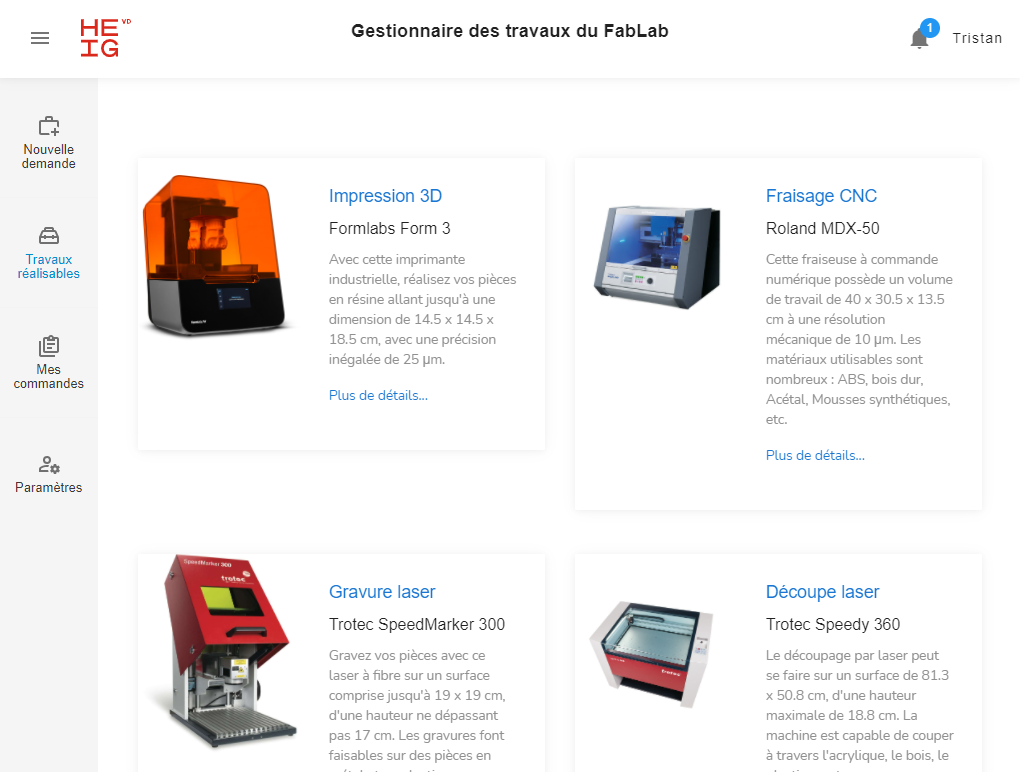
\includegraphics[width=14cm]{ui_joblist_page.PNG}
  \caption{Page "Travaux disponibles" du client}
\end{figure}

La seconde page commune est celle de la liste des demandes, sous l'onglet "Mes commandes". Pour le client, elle contient les demandes qu'il a déposé et pour le technicien, les demandes qui lui sont assignées.

\begin{figure}[h]
  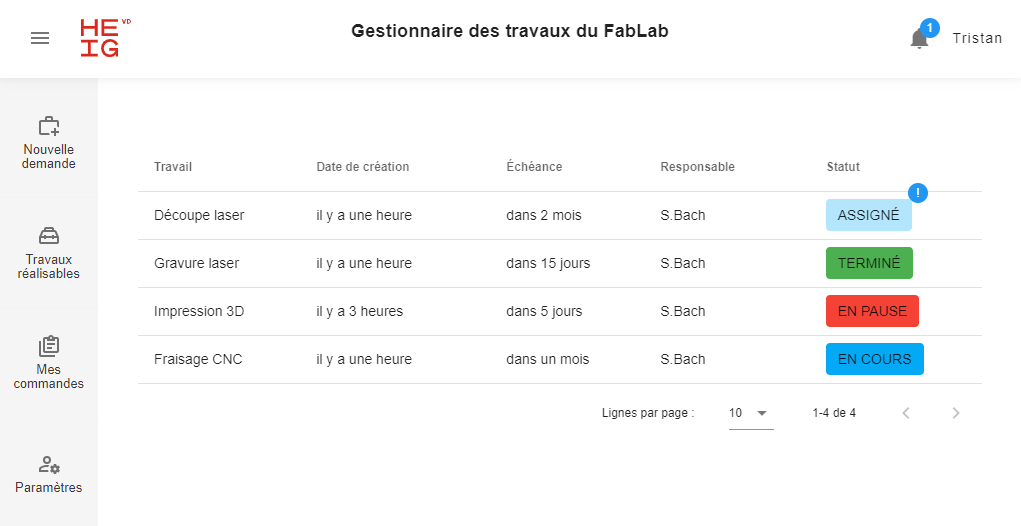
\includegraphics[width=14cm]{ui_myjobs_client.PNG}
  \caption{Page "Mes commandes" du client}
\end{figure}

La table offre la possibilité de trier une colonne à la fois, et par défaut le tri est fait en fonction du statut.
Ce tri par défaut fait en sorte que les demandes notifiées apparaissent toujours en premier. Une demande notifiée est une demande qui possède un point d'exclamation dans sa colonne "Statut".
La cloche de notification indique toujours le nombre de demandes notifiées.

En cliquant sur une des entrées du tableau, la fenêtre des détails va s'ouvrir. Dessus, on retrouve ce qui était prévu dans le croquis. Les détails sont affichés en colonne, en haut de la fenêtre.
Si un commentaire est attaché à la demande, il est affiché quand on clique sur l'icône de la colonne correspondante. Si on clique sur le bouton de la colonne "Fichiers", un menu contenant les noms des fichiers se déroule. Il suffit de cliquer sur un des noms pour lancer le téléchargement du fichier choisi.
Un stepper à 4 étapes indique visuellement l'état d'avancement du travail. En bas à gauche et à droite se situent la chatbox et la timeline.

La chatbox est une fenêtre de chat pour l'échange de messages entre les acteurs. Une bannière délimite les messages par date, et une autre apparait si des nouveaux messages sont présents.
Dans la timeline sont affichés tous les évènements de la demande. C'est depuis ici que peuvent être ajoutés des fichiers. Pour les évènements de type fichier, un numéro de version indique si un fichier a été écrasé. Il n'y a pas de limitations pour l'ajout des fichiers, hormis une limite de 5 MB par envoi.

\begin{figure}[h]
  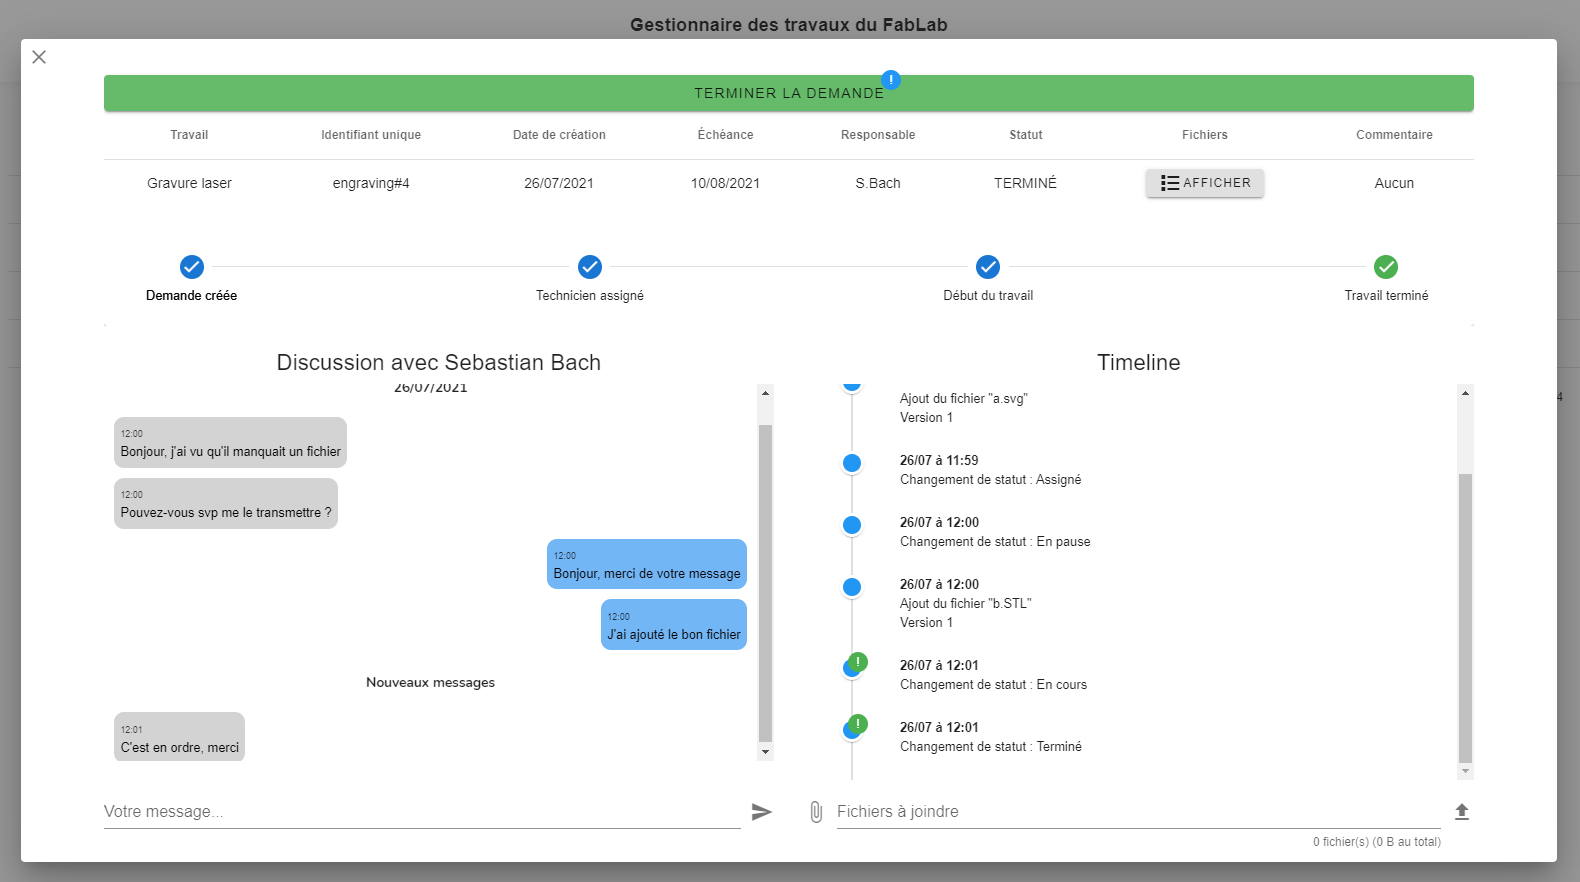
\includegraphics[width=14cm]{ui_jobinfo_client2.PNG}
  \caption{Fenêtre des détails d'une demande terminée, côté client}
\end{figure}

Quand une demande passe au statut "Terminé", le client voit apparaitre un long bouton vert tout en haut de la fenêtre. Ce bouton sert à évaluer le travail et à l'effacer. Une fois validé, le travail disparait pour tout le monde.

\begin{figure}[h]
  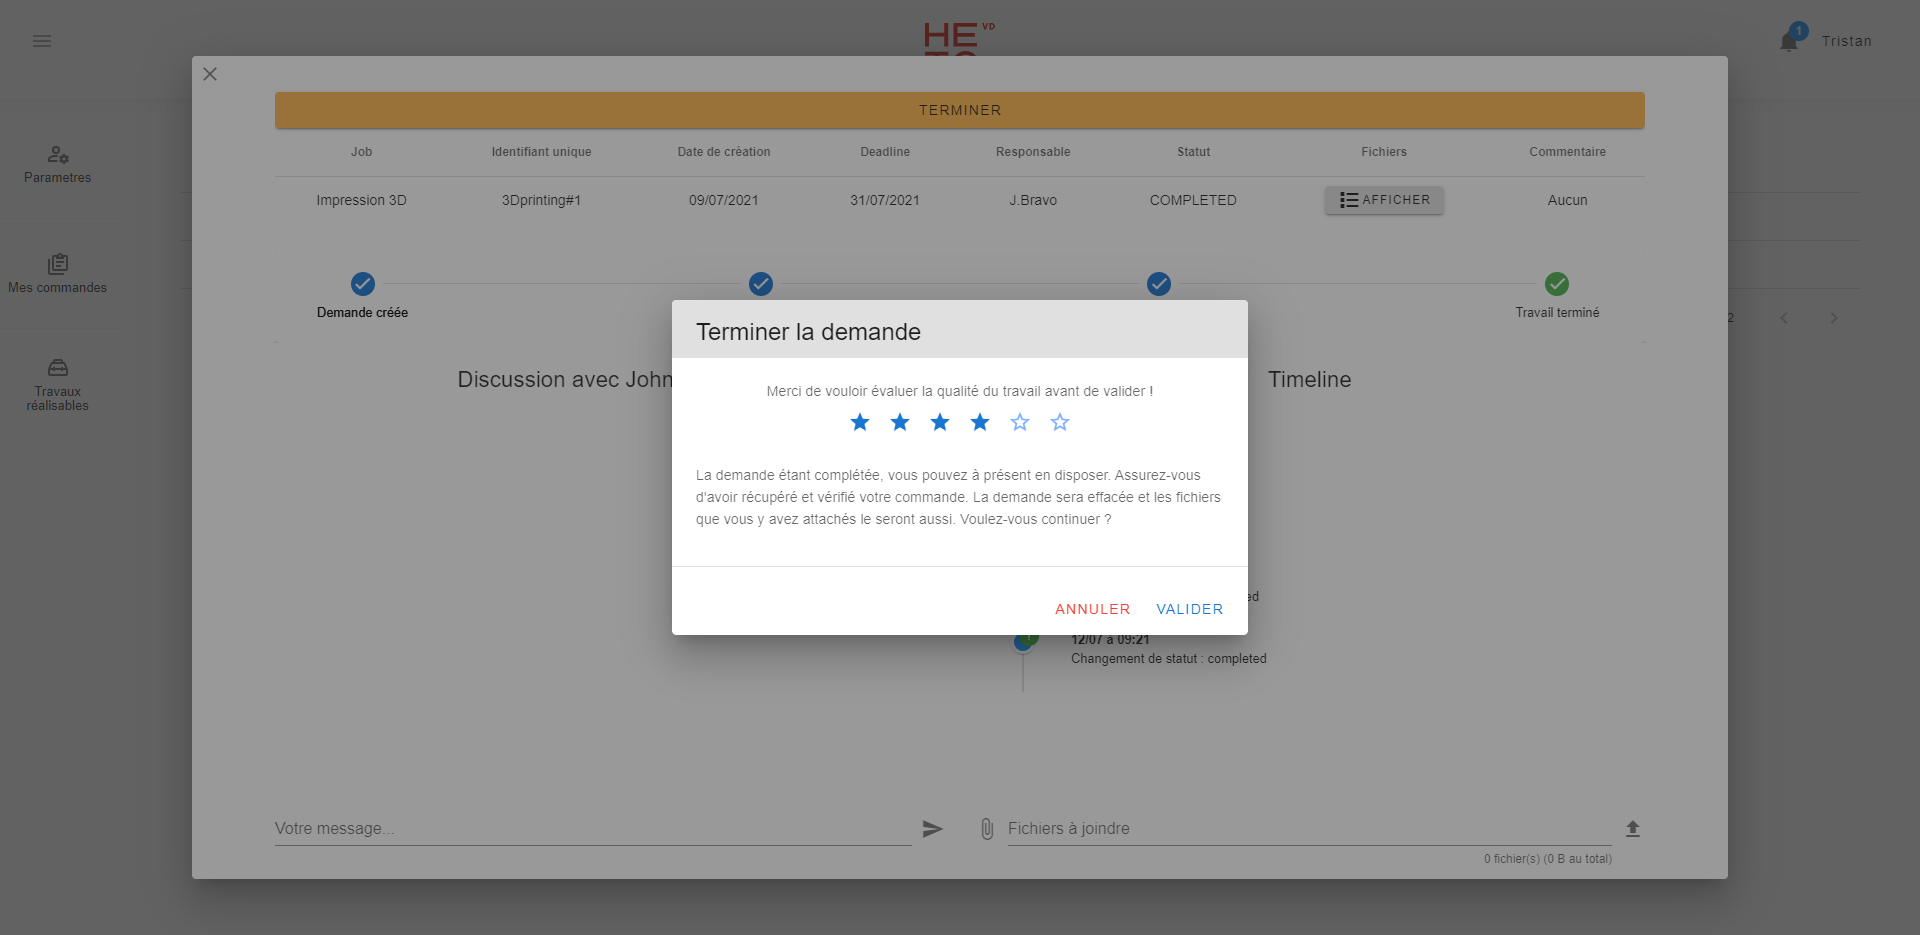
\includegraphics[width=14cm]{ui_jobinfo_client3.PNG}
  \caption{Évaluation et suppression du travail terminé}
\end{figure}

L'alerte de notification pour la demande est retirée dès que la fenêtre des détails est fermée, signifiant que l'utilisateur a vu les changements.

\newpage
Si l'utilisateur est un technicien, une fonctionnalité de plus lui est offerte. Sa colonne "Statut" possède un bouton qui lui permet d'éditer le statut de la demande. Un sélecteur lui permet de choisir le nouveau statut parmi ceux qui sont disponibles. Il ne peut que faire progresser l'avancement de la demande, donc les options qui s'offrent à lui évoluent en fonction du stade actuel. Quand il met le statut "Terminé", il ne peut plus le modifier. La figure \ref{lifecycle.xml} illustre l'ordre des statuts.

\begin{figure}[h]
  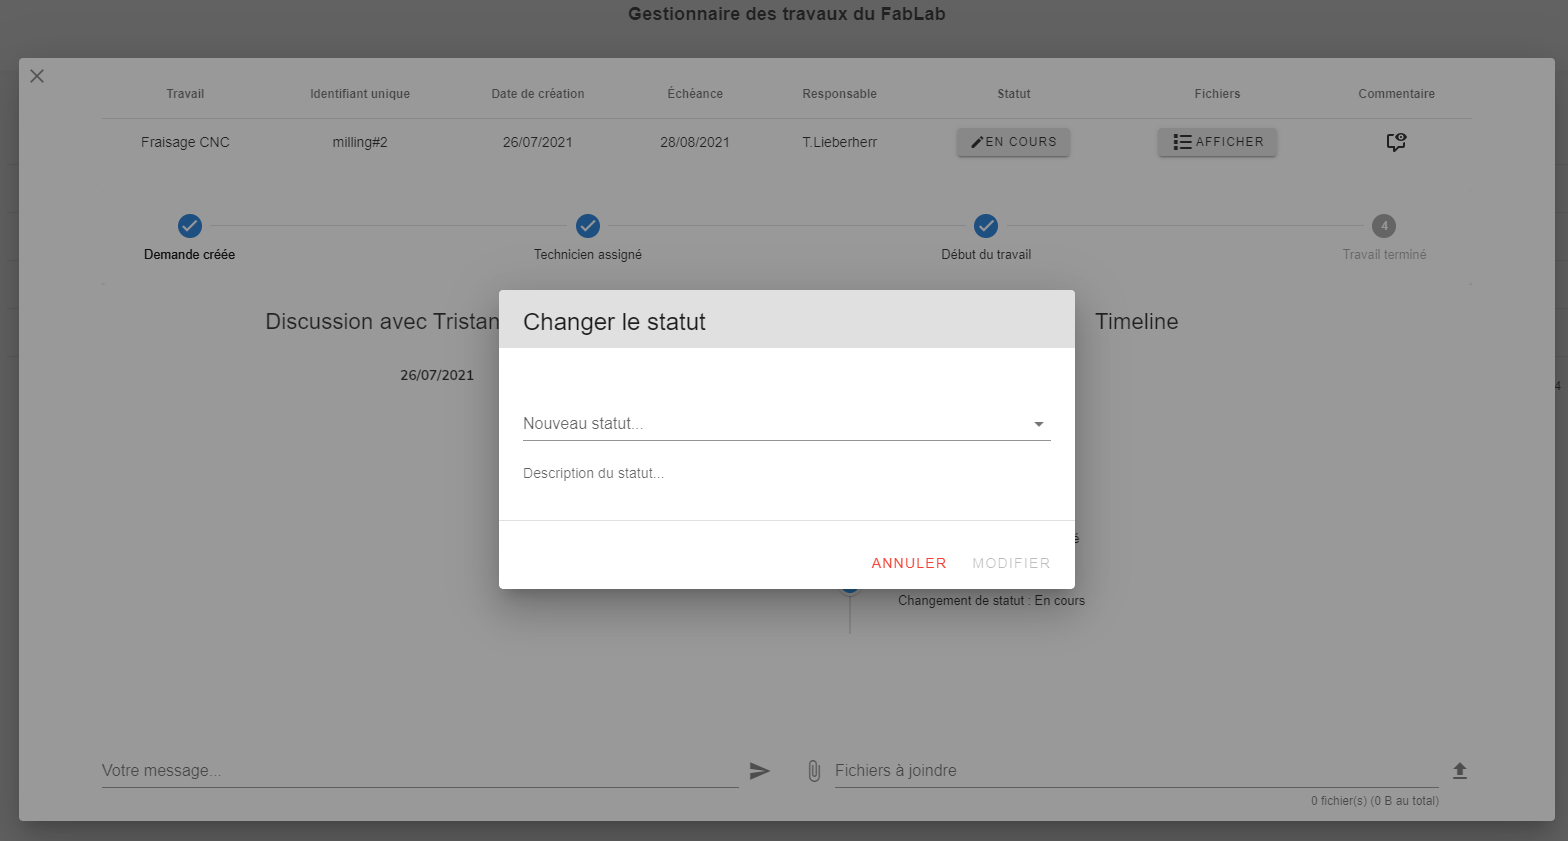
\includegraphics[width=14cm]{ui_jobinfo_tech2.PNG}
  \caption{Modification du statut accessible au technicien}
\end{figure}

\newpage
Si le travail n'est pas encore assigné, la timeline et la chatbox ne sont pas disponibles. Par conséquent, la fenêtre des détails en informe l'utilisateur.
Dès que la demande est assignée, la fenêtre retrouve son affichage normal.

\begin{figure}[h]
  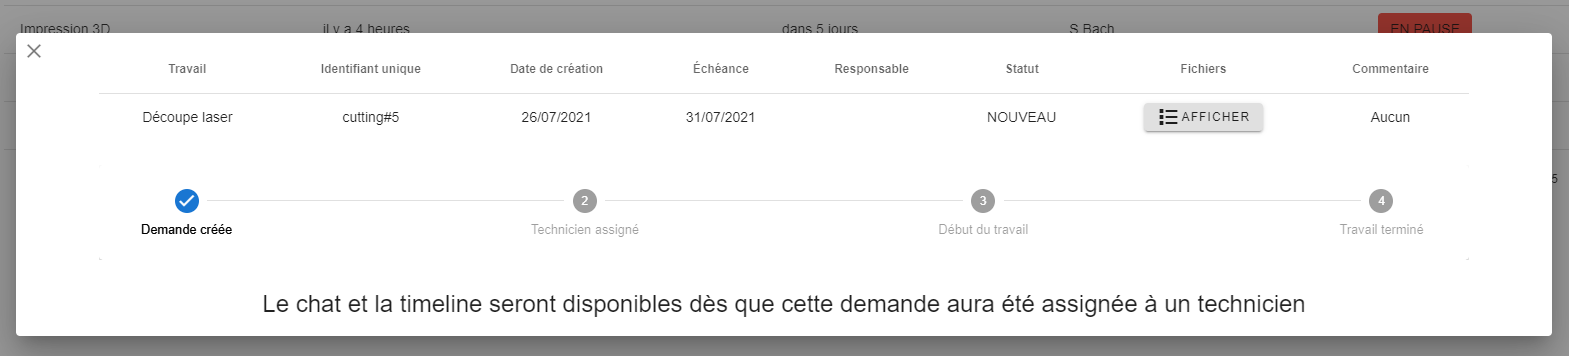
\includegraphics[width=14cm]{ui_jobinfo_client1.PNG}
  \caption{Fenêtre des détails d'une demande non assignée, vu par le client}
\end{figure}

La dernière page commune est celle des paramètres, aussi sous l'onglet du même nom. Elle ressemble beaucoup à ce qui était prévu dans le croquis.
Il y a trois options pour personnaliser l'envoi d'emails de notification. Ces options déterminent quels évènements vont déclencher l'envoi d'un courriel.
Pour les modifier, des switchs sont utilisés. Ils sont avantageux puisqu'ils indiquent directement leur état : ON ou OFF.
Par souci de confort, il est possible d'activer ou de désactiver toutes les options d'un coup, avec le switch "Notifications par mail".

\begin{figure}[h]
  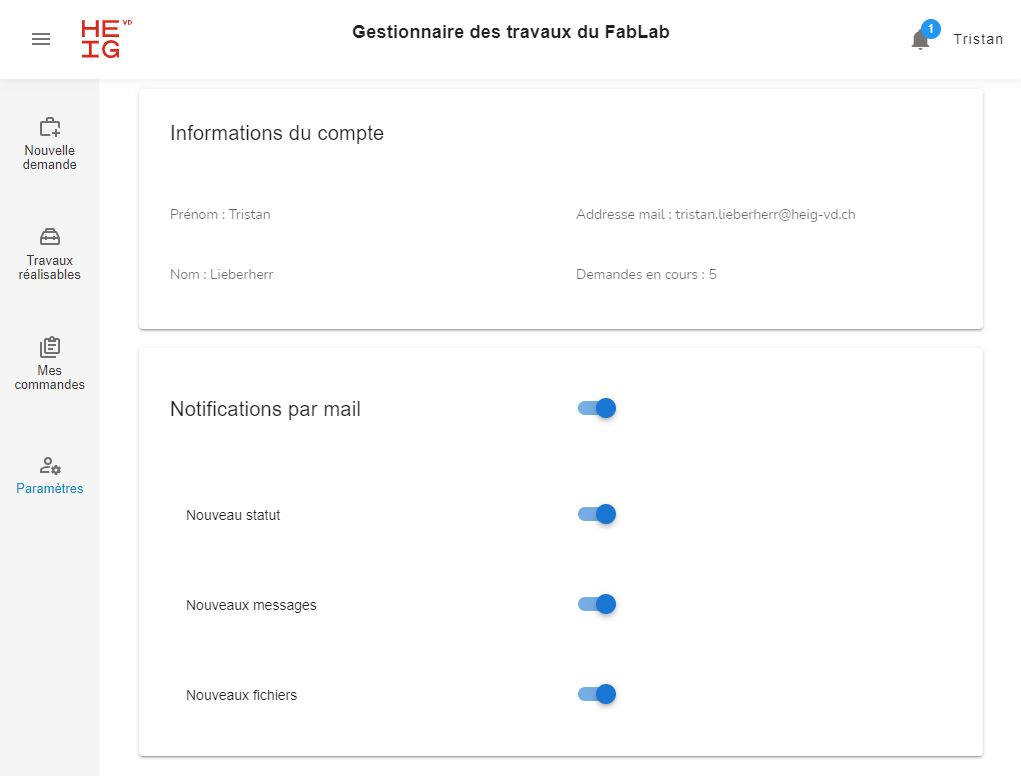
\includegraphics[width=14cm]{ui_settings_page.PNG}
  \caption{Page des paramètres du client}
\end{figure}

Il n'y a pas besoin d'appliquer les modifications, puisqu'elles se font directement lors du changement d'état des boutons : une animation de chargement indique que les modifications sont en train d'être appliquées, ce qui indique à l'utilisateur que les changements sont biens enregistrés.

\newpage
Comme mentionné plus tôt, les clients et les techniciens n'ont pas accès aux mêmes pages et aux mêmes fonctionnalités.

Les clients ont accès au formulaire de nouvelle demande. Ce formulaire est accessible soit depuis la page des travaux disponibles, soit depuis l'onglet "Nouvelle demande".
Un formulaire ouvert depuis l'onglet est totalement vierge. Sur ce formulaire se trouvent tous les champs nécessaires à la création d'une nouvelle demande.

\begin{figure}[h]
  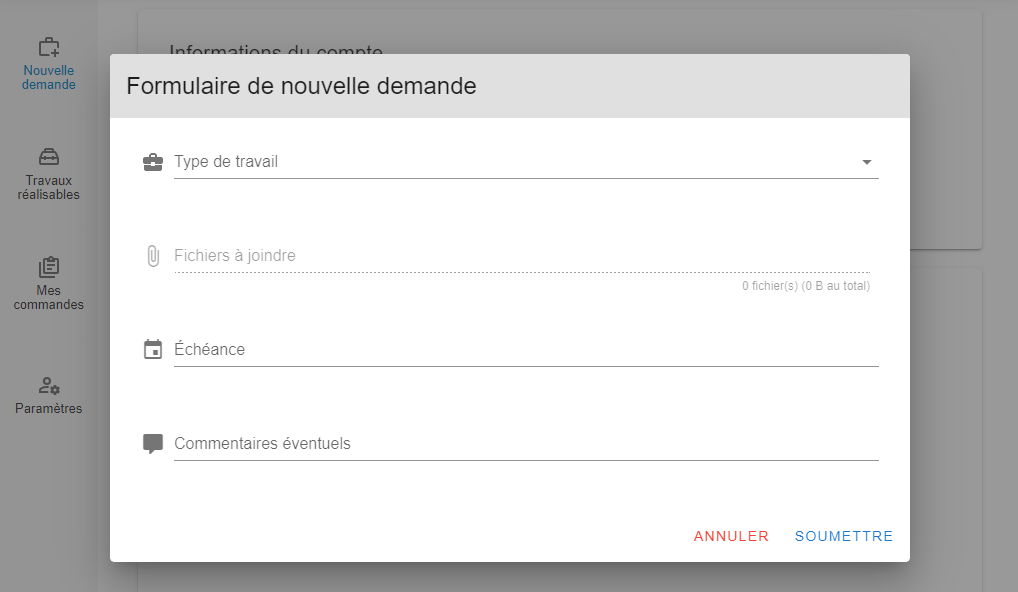
\includegraphics[width=14cm]{ui_submit1.PNG}
  \caption{Formulaire vierge}
\end{figure}

L'utilisateur doit obligatoirement indiquer le type de travail, fournir les fichiers requis et indiquer une date de délai. Le commentaire éventuel est facultatif.
Les types de fichiers requis sont indiqués sous le champ "Fichiers à joindre".

\begin{figure}[h]
  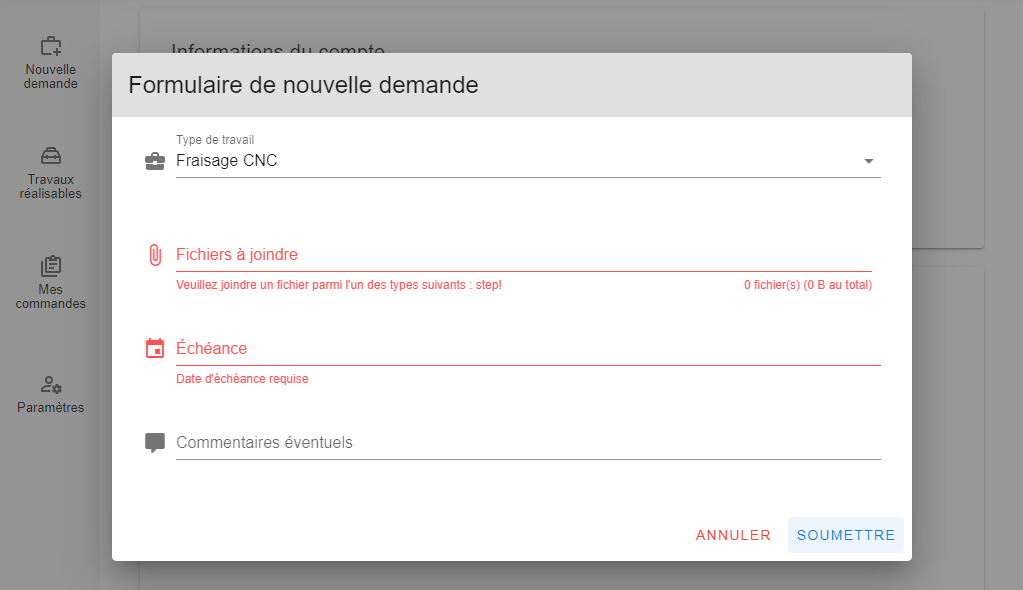
\includegraphics[width=14cm]{ui_submit2.PNG}
  \caption{Formulaire incomplet}
\end{figure}

En cliquant sur le bouton "Soumettre", les champs sont vérifiés et en cas de problème, un message d'erreur apparait sous les champs concernés.
Le formulaire ne peut être envoyé tant que des erreurs persistent. Quand il est finalement envoyé, la nouvelle demande se retrouve tout de suite dans le tableau de la page "Mes commandes".

Les techniciens, quant à eux, ont accès à une page supplémentaire qui contient la liste de toutes les demandes non-assignées, depuis l'onglet "Commandes clients".
Une table contenant tous les travaux non assignés est affichée. Les colonnes indiquent quelques informations de base, et surtout, il y a la possibilité de cocher les demandes. En cochant les demandes, le technicien peut se les assigner, à l'aide du bouton "Assigner". Une confirmation lui est demandée et une fois le choix validé, les travaux sélectionnés disparaissent de la table de tous les techniciens connectés, et le technicien qui s'est assigné les demandes les reçoit dans sa table de la page "Mes commandes".
Chaque fois qu'une nouvelle demande est déposée par un client, tous les techniciens peuvent la voir en temps réel depuis ce tableau.

\begin{figure}[h]
  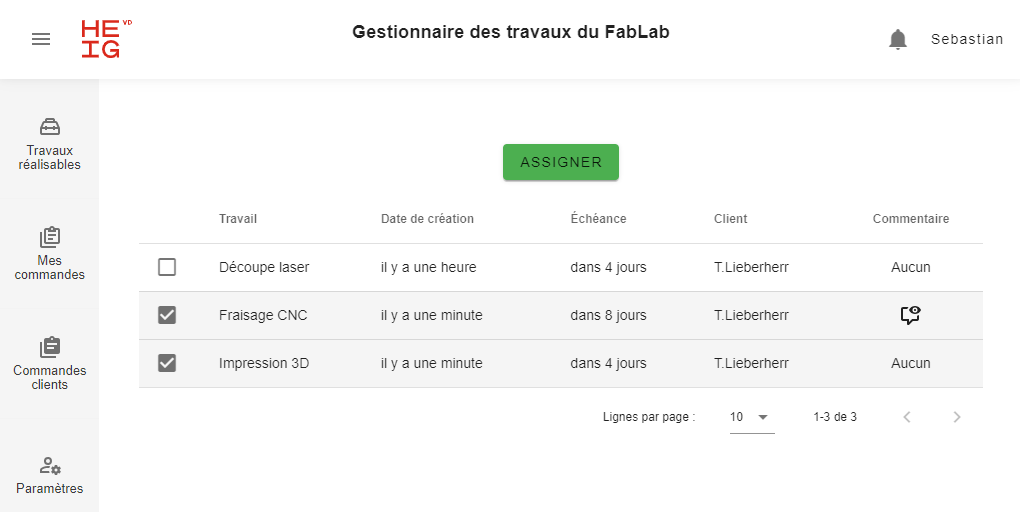
\includegraphics[width=14cm]{ui_alljobs_page.PNG}
  \caption{Table des demandes non-assignées du technicien}
\end{figure}

\begin{figure}[h]
  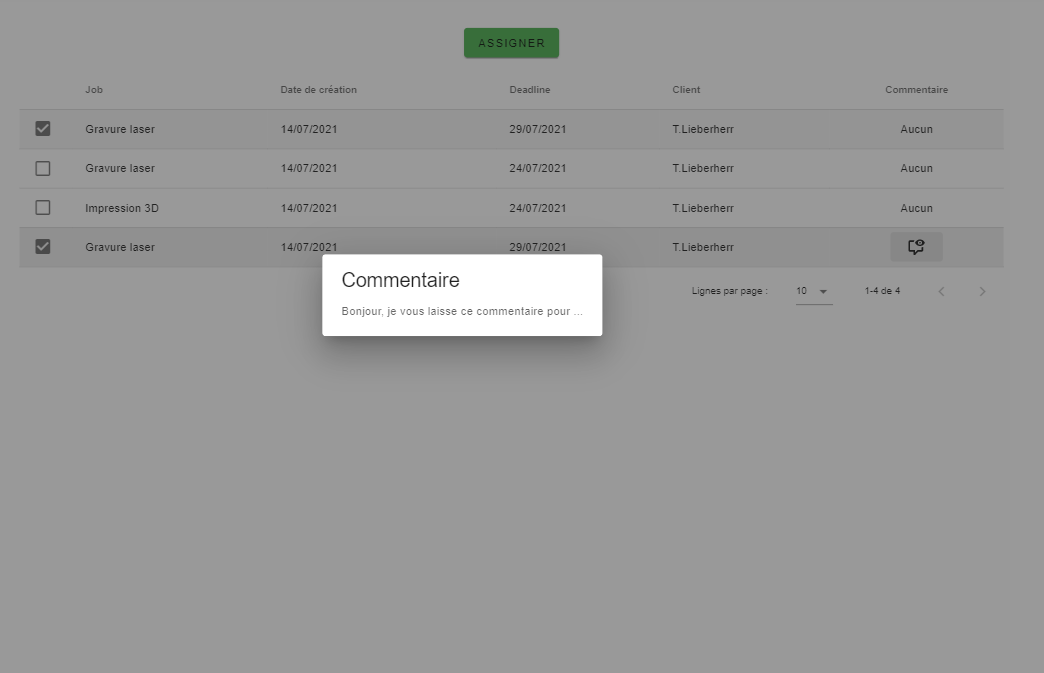
\includegraphics[width=14cm]{ui_alljobs_comment.PNG}
  \caption{Affichage du commentaire}
\end{figure}

\newpage
\section{Interface pour mobiles}
L'interface web étant réactive, elle doit être adaptée à un usage sur mobile. Les fonctionnalités offertes sont identiques que sur la version PC : le seul changement est l'affichage.
Grâce aux nombreux composants de la bibliothèque Vuetify et de la structure initiale du site, l'affichage adaptatif pour mobile était presque toujours fonctionnel. Il m'a tout de même fallu apporter des changements pour corriger certains problèmes d'affichage.

Le développement a été fait avec l'aide de la console Chrome, en utilisant l'appareil virtuel Moto G4 de 360 x 640 pixels. Les vérifications ont été faites en parallèle depuis mon Samsung S8.

\begin{figure}[h]
  \centering
  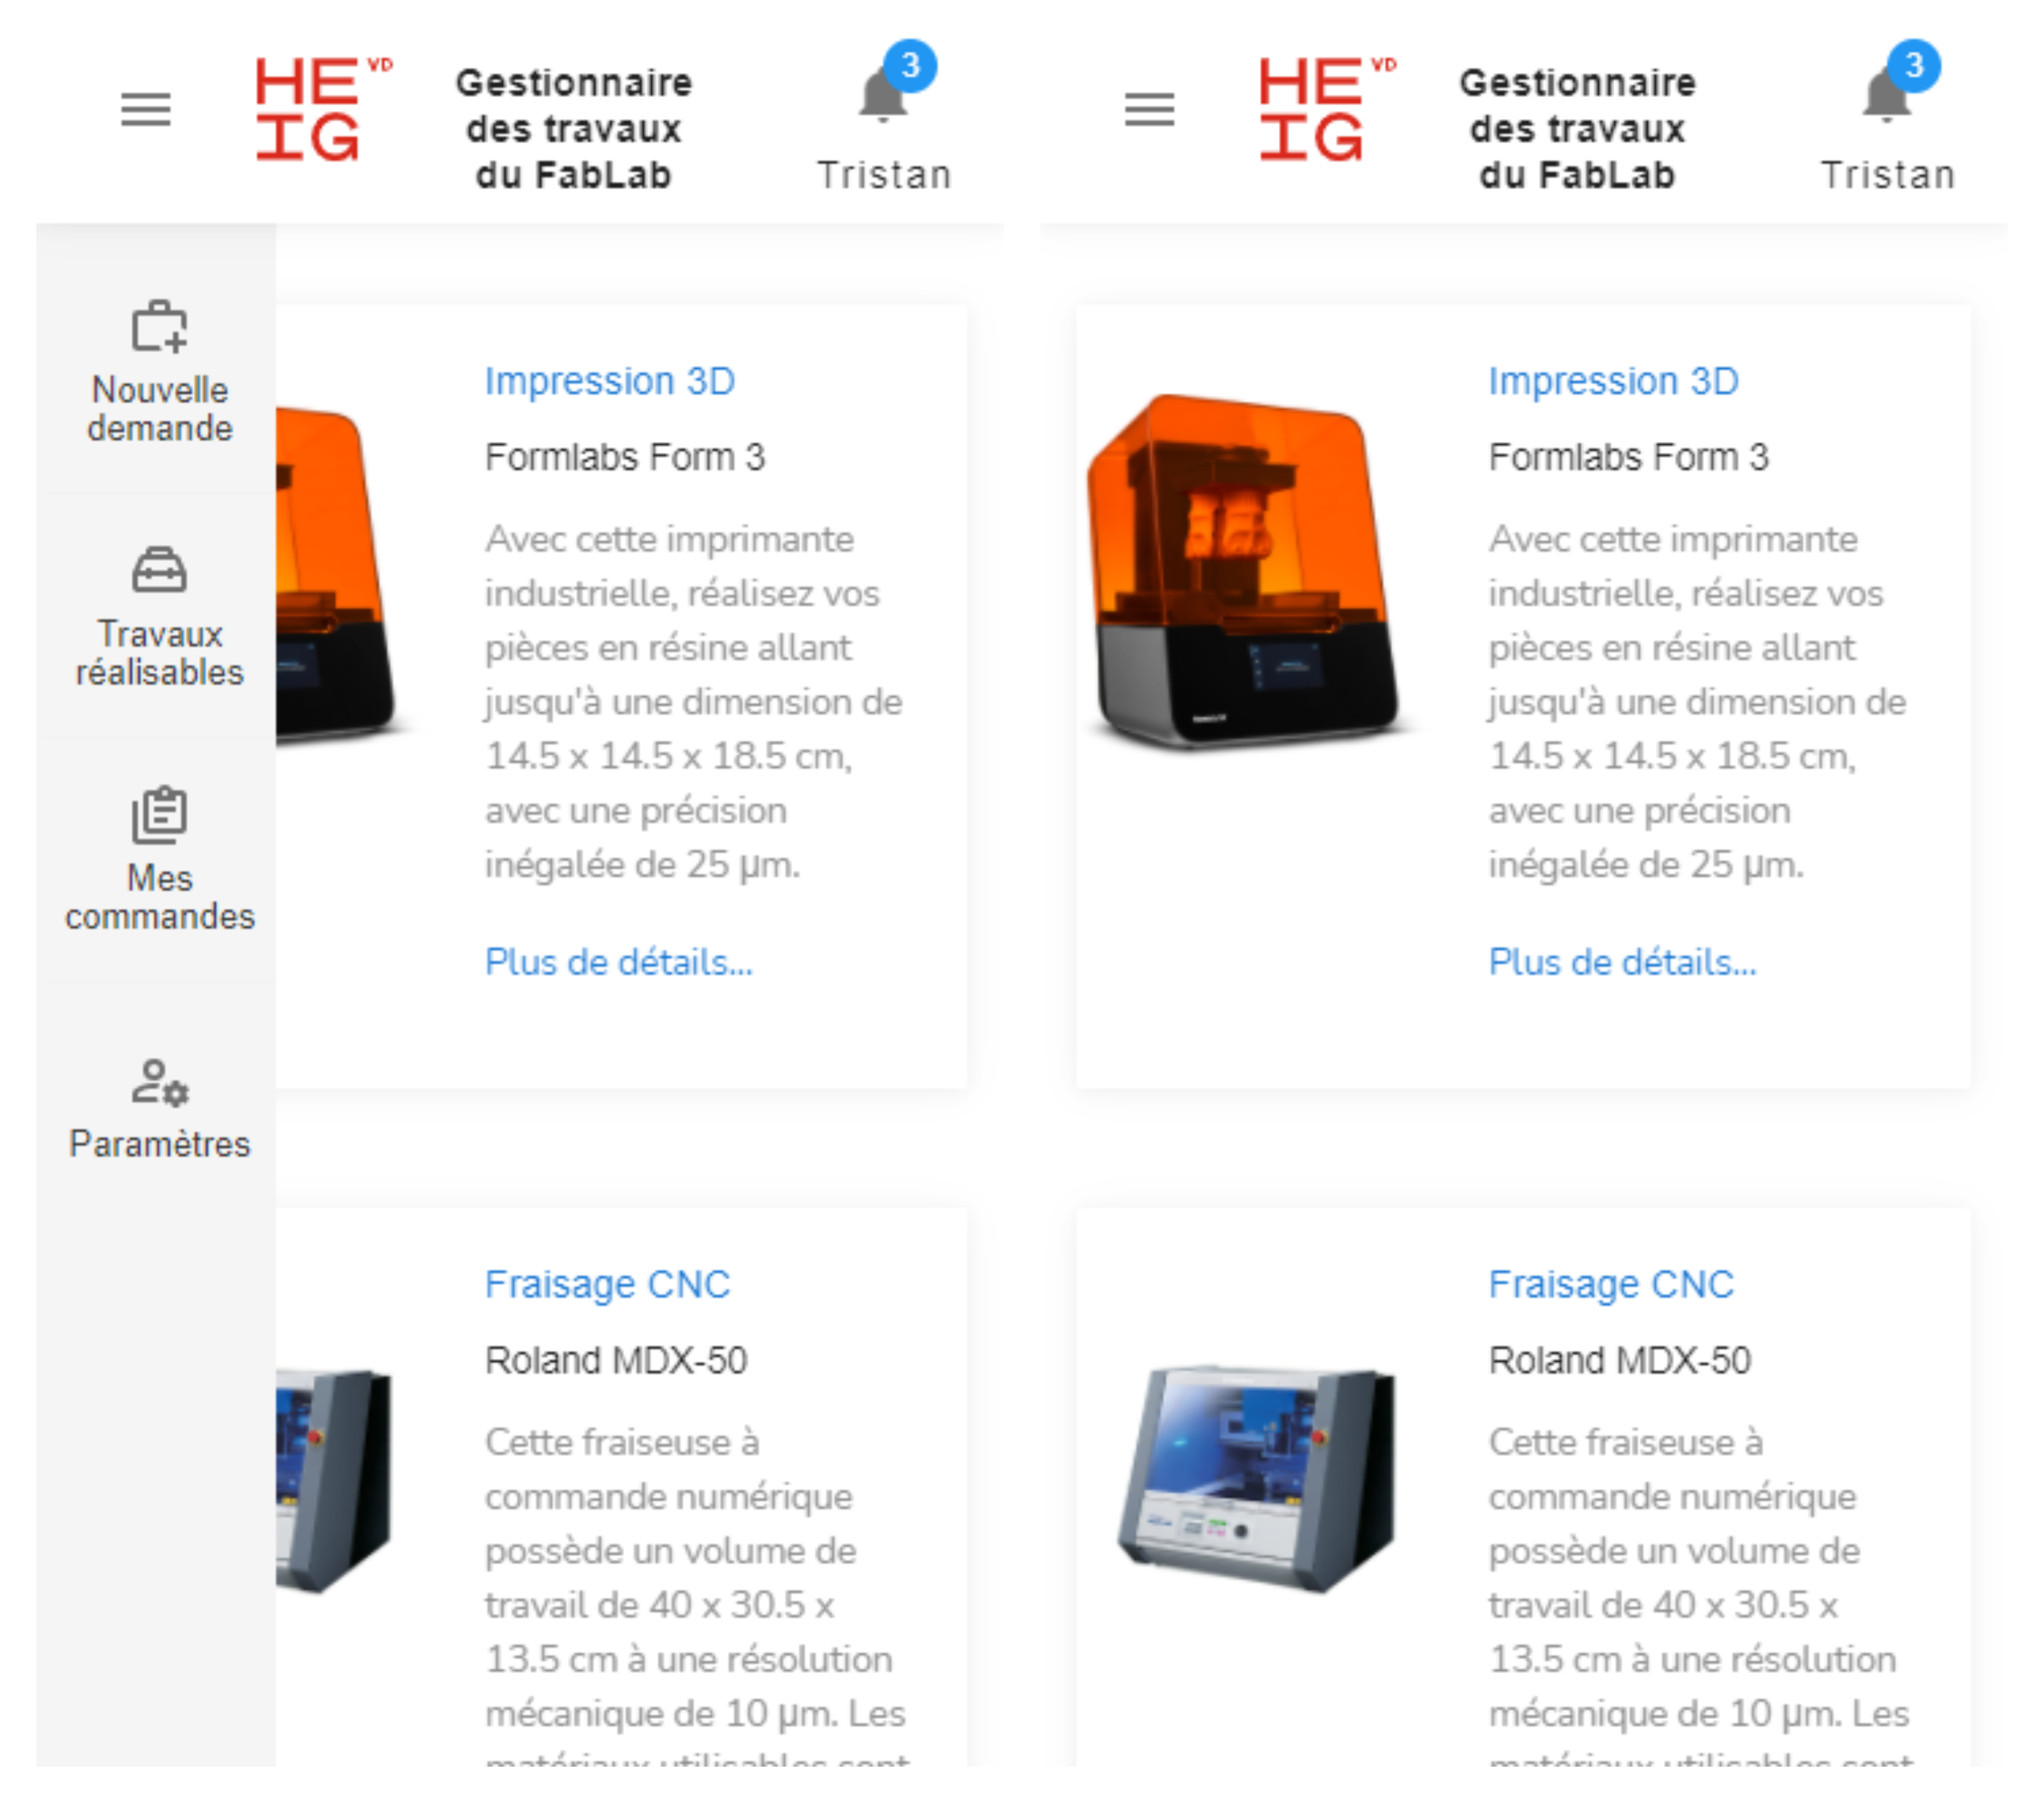
\includegraphics[width=12cm]{ui_mobile_joblist_portrait.PNG}
  \caption{Barre latérale en mode portrait et liste des travaux disponibles}
\end{figure}

La barre latérale recouvre désormais le contenu des pages. Le contenu de la barre du haut change aussi pour pouvoir garder tous les éléments à l'écran. Ces derniers sont néanmoins assez éloignés les uns des autres pour ne pas cliquer sur l'élément voisin.
Pour la page des travaux disponibles, au lieu d'une liste à deux colonnes, il n'en reste qu'une, suffisamment large pour afficher le contenu.

\newpage
Les tables aussi sont changées. En mode portrait, les lignes prennent la forme d'une liste, et le tri se fait depuis un sélecteur. Le fonctionnement est sinon identique.

\begin{figure}[h]
  \centering
  
\includegraphics[width=11cm]{ui_mobile_landscape.PNG}
  \caption{Barre latérale en mode paysage}
\end{figure}

\begin{figure}[h]
  \centering
  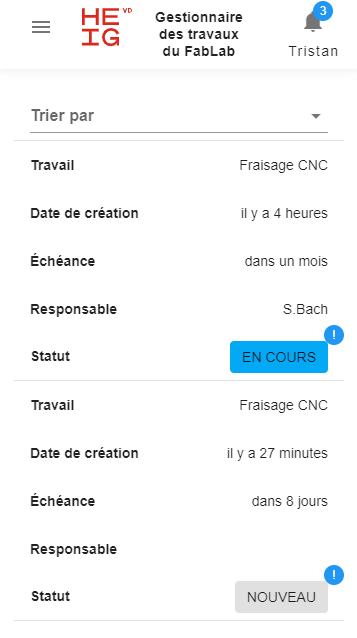
\includegraphics[height=10cm]{ui_mobile_myjobs_client_portrait.PNG}
  \caption{Table des demandes du client, mode portrait}
\end{figure}

\newpage
En mode paysage, la forme est similaire que sur PC. L'avantage est qu'il y a la possibilité de changer d'orientation pour changer l'affichage des tables.

\begin{figure}[h]
  \centering
  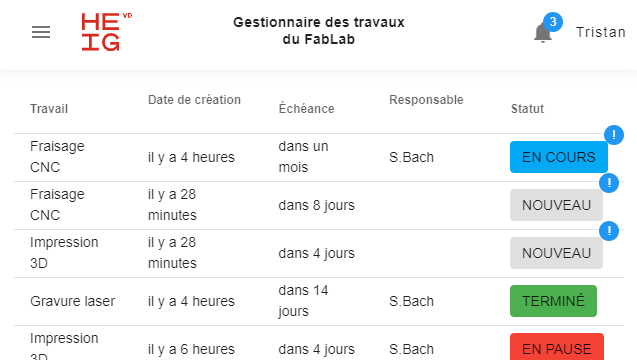
\includegraphics[width=11cm]{ui_mobile_myjobs_client_landscape.PNG}
  \caption{Table des demandes du client, mode paysage}
\end{figure}

\begin{figure}[h]
  \centering
  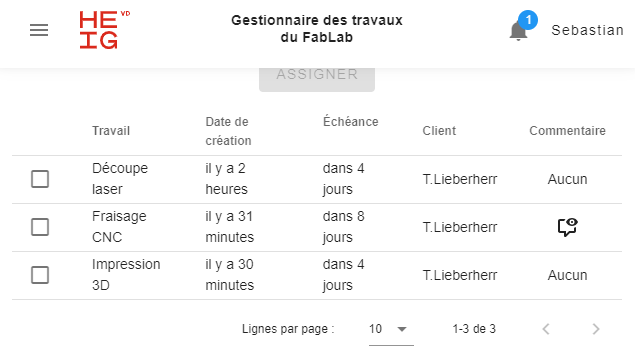
\includegraphics[width=11cm]{ui_mobile_alljobs_landscape.PNG}
  \caption{Table des demandes non-assignées, mode paysage}
\end{figure}

Le composant qui change radicalement de forme est la fenêtre des détails. Vu qu'il n'y a pas la place pour l'afficher en entier sur un écran de smartphone, j'ai décidé de mettre un carousel de 4 fenêtres à la place. Il y a une fenêtre pour les détails, une pour le stepper, une pour la timeline et une pour la chatbox. L'utilisateur peut naviguer entre ces vues en swipant du doigt.
Si la demande n'est pas encore assignée, les fenêtres de la chatbox et de la timeline ne sont pas présentes.

\newpage

\begin{figure}[h]
  \centering
  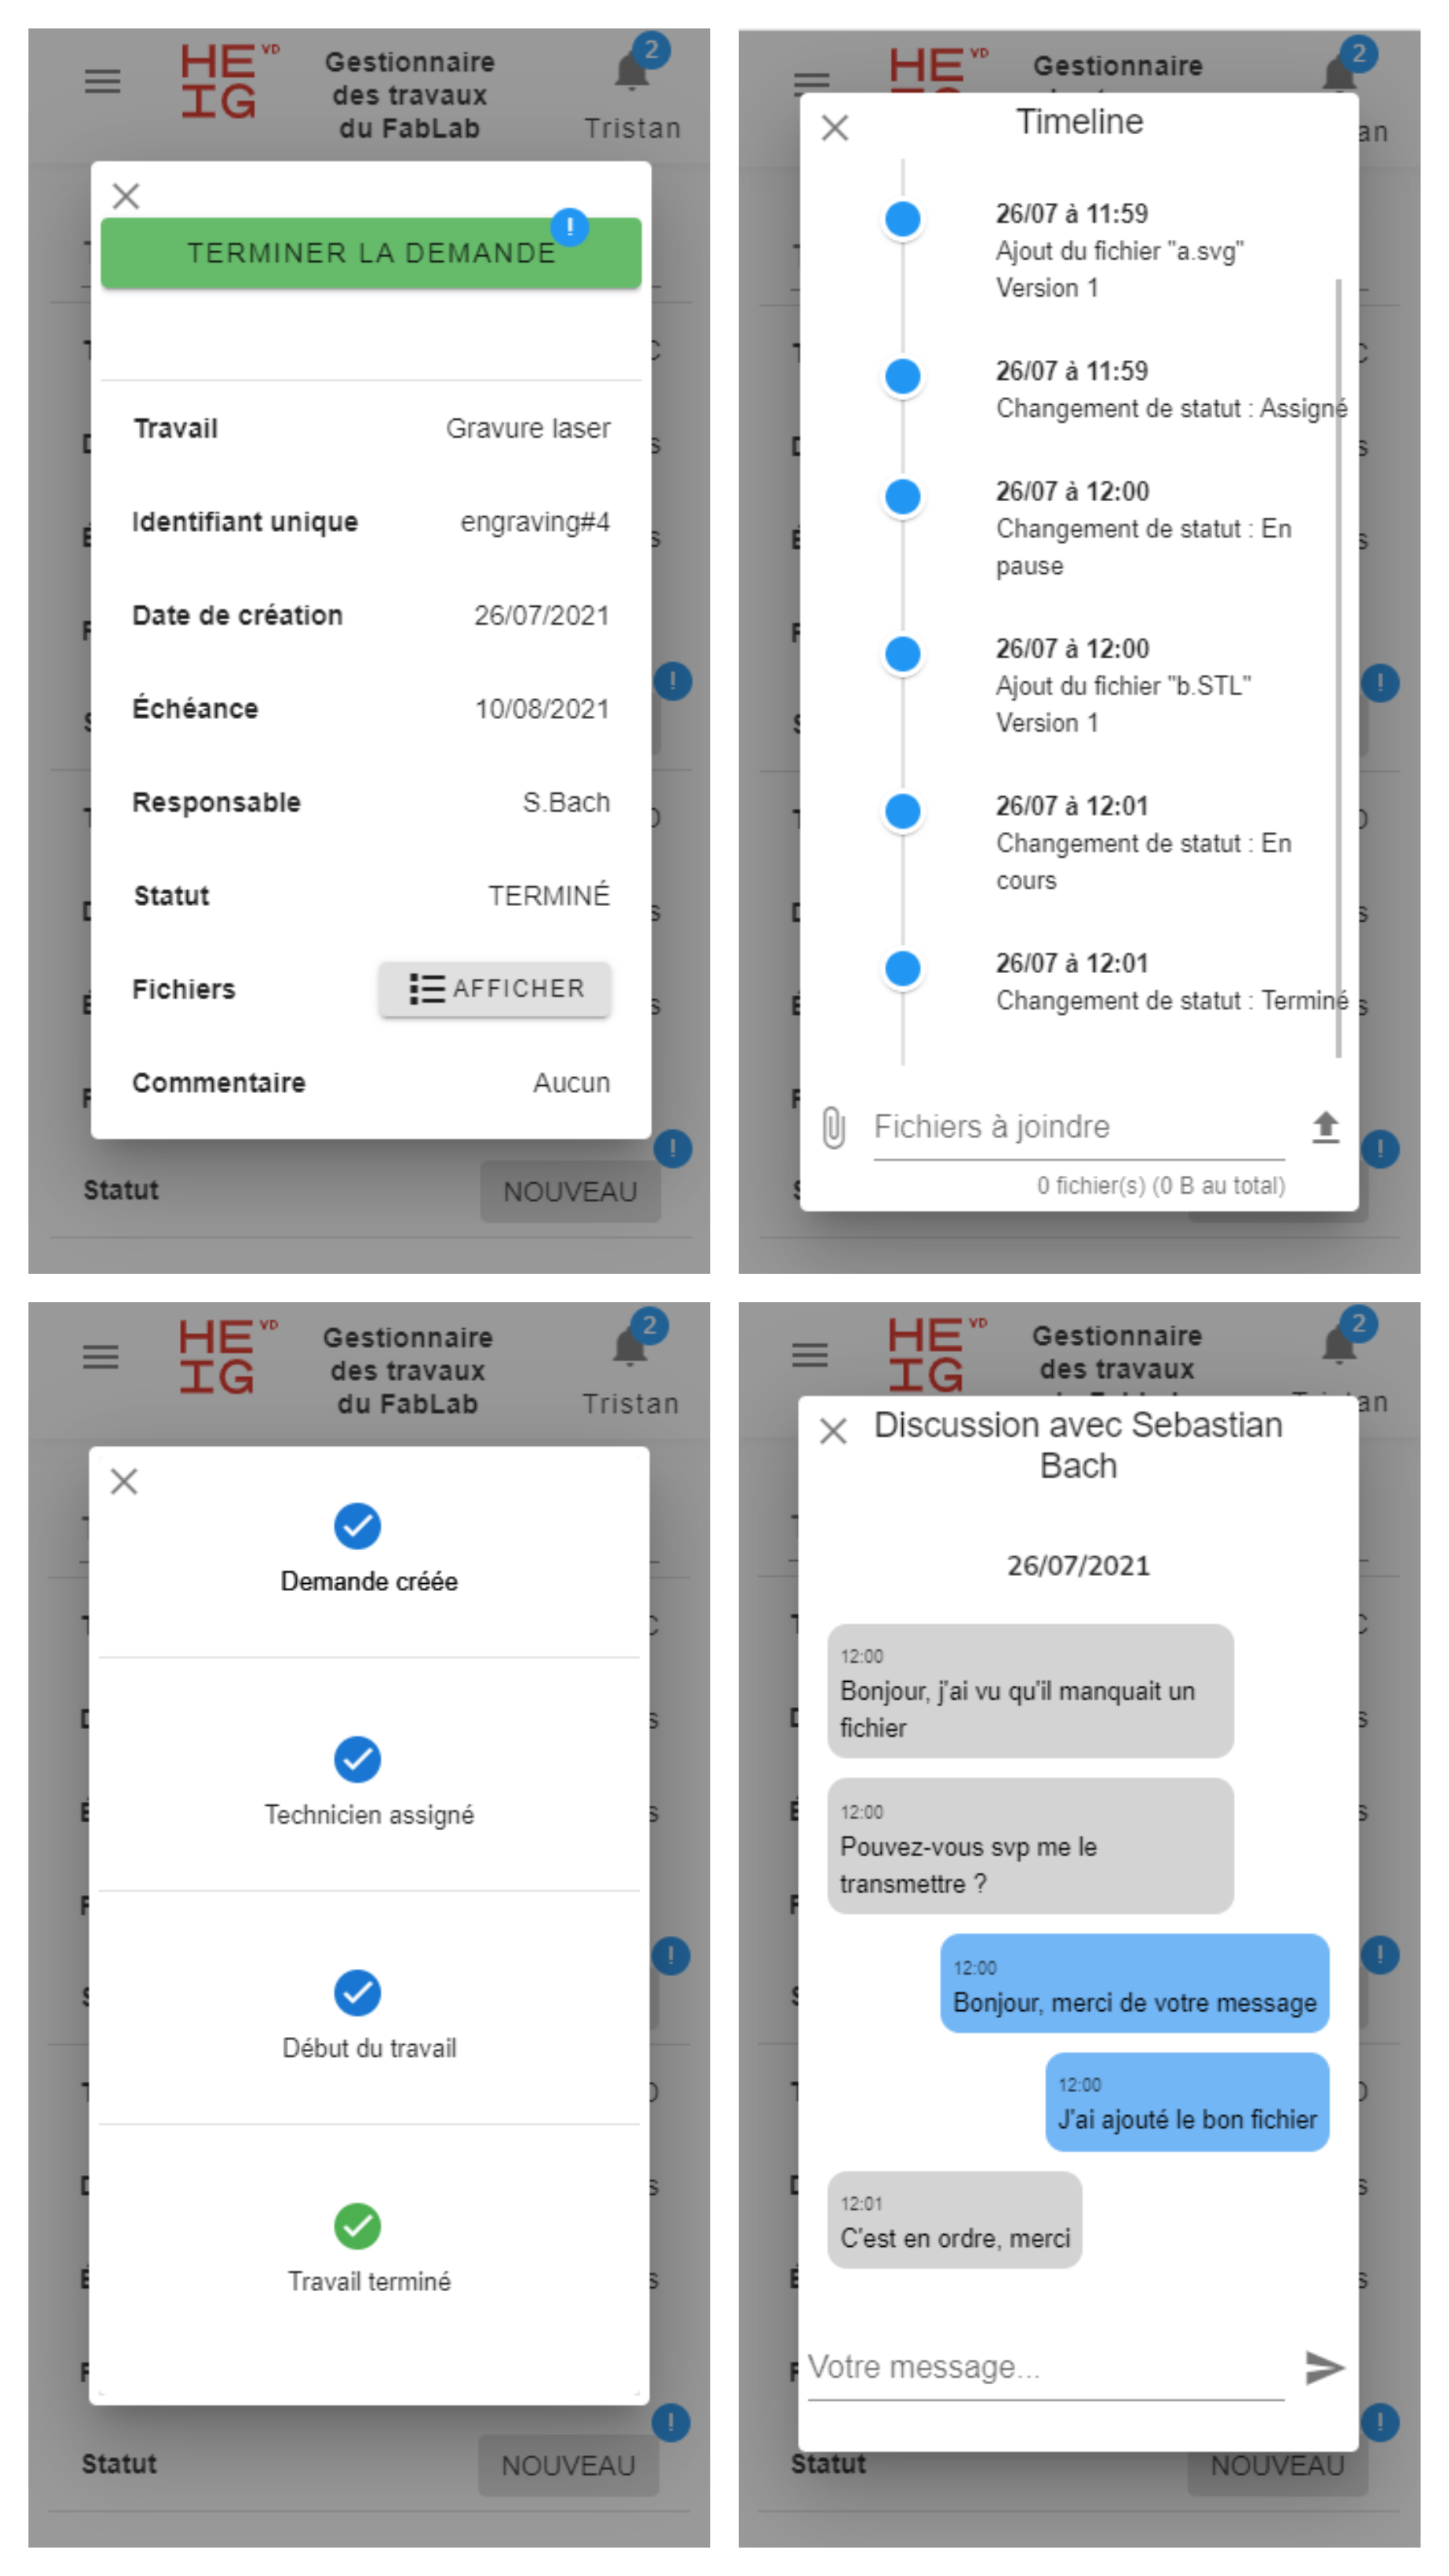
\includegraphics[width=10cm]{ui_mobile_jobinfo.png}
  \caption{Carousel des détails d'une demande du client, mode portrait}
\end{figure}

\newpage
\section{Routage}
Le frontend possède une liste de routes internes qui mènent chacunes à une page différente. C'est le routeur de la SPA qui s'occupe d'intercepter ces routes et d'afficher la bonne page.

Le fichier "router.js" contient une représentation objet de ces routes. Chaque nom de route, signalée par "path", possède une vue (une page) associée, "component". L'utilisation d'un tableau "children" permet d'imbriquer des routes.

\begin{figure}[h]
  \begin{minted}[breaklines]{javascript}
  const routes = [
    {
      path: "/",
      redirect: "/app",
    },
    {
      path: "/app",
      component: () => import("./views/app"),
      redirect: "/app/my-jobs",
      children: [
        {
          path: "my-jobs", //page "Mes commandes"
          component: () => import("./views/app/myJobs/MyJobs"),
        },
        {
          path: "all-jobs", //page "Commandes clients"
          component: () => import("./views/app/myJobs/AllJobs"),
          beforeEnter: (to, from, next) => {
            next(store.getters.getUser.is_technician ? {} : '/')
          }
        },
        {
          path: "job-list", //page "Travaux réalisables"
          component: () => import("./views/app/jobList/JobList"),
        },
        {
          path: "settings", //page "Paramètres"
          component: () => import("./views/app/settings/Settings"),
        },
      ]
    },
    {
      path: "*", //page 404
      component: () => import("./views/Error")
    }
  ];
  \end{minted}
  \caption{router.js}
\end{figure}

Un garde de navigation, utilisé sur la route "all-jobs", permet de rediriger une route sous certaines conditions. En l'occurence, il faut que l'utilisateur soit un technicien, sans quoi il est redirigé ailleurs. La vérification de l'authentification ne se fait pas à ce niveau : ce sujet est traité dans un des chapitres suivants.

\newpage
Si on organise ces routes sous forme de liste, on obtient la chose suivante :
\begin{itemize}
  \item '/' : redirige sur /app (puis sur /app/my-jobs)
  \item '/app' : racine de la SPA. Cette route toute seule redirige sur /my-jobs
  \item '/app/my-jobs' : page "Mes commandes"
  \item '/app/all-jobs' : page "Commandes clients", accessible seulement aux techniciens. Si un client tente d'y accéder, il est redirigé sur "/"
  \item '/app/job-list' : page "Travaux réalisables"
  \item '/app/settings' : page "Paramètres"
  \item '/*' : toutes les routes indéfinies finissent ici, sur la page 404
\end{itemize}
\bigskip

Si une route n'est pas trouvée, la ravissante page 404 apparait. Le bouton "Retour" redirige l'utilisateur sur la route "/". Au final, il est envoyé sur la page "Mes commandes".

\begin{figure}[h]
  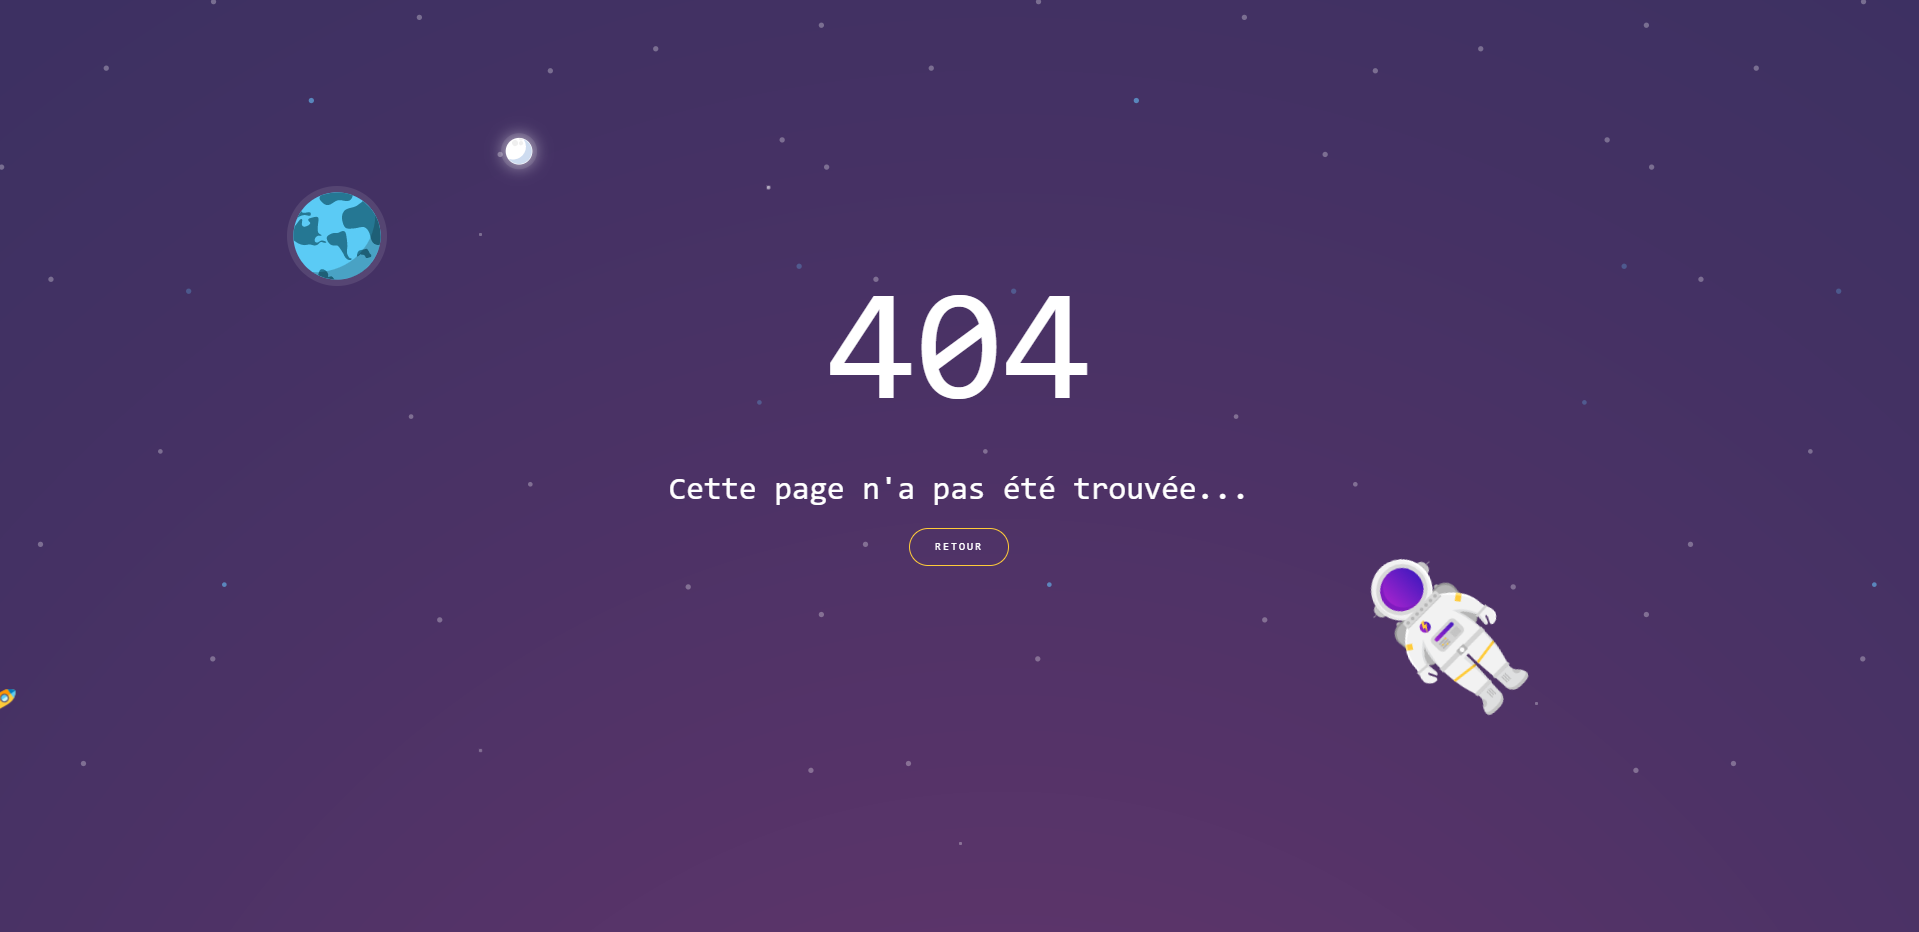
\includegraphics[width=14cm]{ui_404.PNG}
  \caption{Page 404}
\end{figure}


\newpage
\section{Gestion des données et pattern MVC}
%% https://code-cartoons.com/a-cartoon-guide-to-flux-6157355ab207
La gestion des données est un aspect très important du frontend.
Pour ce faire, il existe un design pattern très populaire qui s'appelle le MVC, pour \emph{Model View Controller}.
Ce pattern est constitué de trois axes :
\begin{enumerate}
  \item Contrôleur : c'est la partie qui gère les interactions entre l'utilisateur et les données
  \item Modèle : c'est les données qui vont être affichées
  \item Vue : c'est l'interface visuelle qui présente les données
\end{enumerate}
\bigskip

Ce pattern est assez simple en terme de fonctionnement, mais il est redoutablement efficace.

\figi{MVC.xml}{14cm}{Pattern MVC}

Comme le site est de type SPA, les données nécessaires à l'affichage sont demandées au serveur par le client.
Il doit donc y avoir un endroit où les stocker : c'est là qu'intervient Vuex.
Le partage de données entre composants est un possibilité, mais Vuex offre bien trop d'avantages.

Vuex est un pattern et une librairie qui fait office de gestionnaire d'état pour les applications Vue.
Plus précisément, c'est un lieu de stockage qui peut contenir des données, rangées dans le "state", et qui offre des accesseurs et des mutateurs pour interagir avec.
Des fonctions sont aussi mises à disposition, et s'appellent des "actions". Tous ces composants font partie du "store".

Le premier avantage de ce système est qu'il n'y a qu'une seule instance des objets stockés dedans, une seule source de vérité accessible depuis tous les composants.
Dans Vue, les composants s'échangent des données soit par props soit par évènements.
Imaginons le cas de figure où le composant G doit accéder à une ressource qui est stockée dans le composant D.
Cette configuration peut poser de gros problèmes, car les données transitent partout et il y a des dépendances entre composants.

\newpage
\figi{vuex1.xml}{14cm}{Échange de données entre composants}

Le problème principal est que plusieurs variables risquent de posséder plusieurs états différents (des valeurs différentes) alors qu'elles devraient partager le même.
La compagnie Facebook a justement eu ce souci il y a quelques années, comme expliqué plus en détails sur \href{https://code-cartoons.com/a-cartoon-guide-to-flux-6157355ab207}{ce site}.
Un bug s'est manifesté sous forme de notifications "fantômes", qui indiquaient de nouveaux messages alors que ce n'était en réalité pas le cas.
Les développeurs ont alors décidé de se débarasser du problème en créant Flux, un nouveau design pattern de gestion d'état, qui a inspiré Vuex par la suite.

\figi{vuex2.xml}{14cm}{Échange de données avec le store}

Avec Vuex, il n'y a pas de problème d'états différents, puisqu'il n'existe qu'un seul exemplaire de la ressource, qui est directement accessible.
Si un composant veut modifier l'état d'une ressource du store, il doit passer par un mutateur et tout changement sera propagé aux composants qui en dépendent.

\newpage
L'utilisation de mutateurs assure que les données soient modifiées de façon synchrone, contrôlée et prédictible.
Les actions servent principalement à envoyer des requêtes au serveur pour y récupérer des données.
Sur le schéma ci-dessous, on voit le cycle qui se produit lorsqu'un composant a besoin de récupérer des données depuis le serveur.
Il appelle une action qui va s'occuper de la requête et de la mutation de la ressource.

\figi{vuex.xml}{14cm}{Fonctionnement des actions du store}

Le second avantage est que toute la partie du code qui s'occupe des requêtes HTTP est située dans les actions, ce qui fait que le code est à portée de main dans un seul fichier.
L'utilisation de Vuex a donc été très utile, surtout pour l'organisation du code et des données, et de l'application efficace du pattern MVC.
De plus, il y a la garantie qu'il n'y aura jamais de problèmes avec l'état des variables entre composants.

Le state de l'application contient quelques variables qui doivent être accessibles depuis tous les composants. La portion de code suivante est tirée du fichier "store/index.js", qui est le fichier qui contient tout le store.

\newpage
\begin{figure}[h]
  \begin{minted}[breaklines]{javascript}
  state: {
    user:
    JSON.parse(document.querySelector("meta[type='user']").getAttribute("value")), //infos de l'utilisateur, disponibles au démarrage dans le code HTML
    jobs: [], //travaux déposés/assignés
    unassignedJobs: [], //travaux non-assignés
    formData: { //variable utilisée pour pouvoir ouvrir le formulaire depuis n'importe quelle page
      dialog: false, //affichage de la fenêtre modale du formulaire
      initialJob: null, //pour pré-remplir le formulaire avec le bon type de travail
    },
  },
  \end{minted}
  \caption{index.js, state du store}
\end{figure}

Lors du démarrage de la SPA, il faut que l'application se connecte au serveur websocket, pour reçevoir les notifications push du serveur.
Les détails du serveur websocket ne seront pas traités dans ce chapitre. Laravel Echo est la librairie JavaScript qui est utilisée dans ce projet.

La réception de données par notification se fait via des canaux. Quand un client (désormais dans le sens client-serveur) se connecte à un canal, il va reçevoir tout ce que le serveur va diffuser dessus. Du point de vue du client, de la SPA dans ce cas, il faut s'abonner à un canal et associer une fonction callback à un évènement. Sur un canal, il peut y avoir plusieurs types d'évènements, qui peuvent être capturés par la fonction appellée à chaque fois que l'évènement a lieu, donc quand le serveur diffuse. Les données transmises du serveur au client circulent au format JSON.

\begin{figure}[h]
  \begin{minted}[breaklines]{javascript}
    window.Pusher = require('pusher-js')
      window.Echo = new Echo({
        broadcaster: 'pusher',
        key: '23d1749ad2b7bf6d3315',
        wsHost: window.location.hostname,
        wsPort: 6001,
        wssPort: 6001,
        forceTLS: true,
        disableStats: true,
        encrypted: true,
        enabledTransports: ['ws', 'wss'],
      })
      let id = this.state.user.id
      window.Echo.channel('message.channel.' + id).listen('MessagePusherEvent', (e) => {
        this.commit("addMessage", e.message)
      })
      window.Echo.channel('job.channel.' + id).listen('JobPusherEvent', (e) => {
        if ('terminated' in e.job) this.commit("removeJob", e.job)
        else this.commit("addOrUpdateJob", e.job)
      })
      if (this.state.user.is_technician) {
        window.Echo.channel('job.channel.0').listen('JobPusherEvent', (e) => {
          this.commit("addOrRemoveUnassignedJob", e.job)
        })
      }
  \end{minted}
  \caption{index.js, action "pusherConnect()"}
  \label{figure:pusherConnect}
\end{figure}

\newpage
La portion du code frontend à la figure \ref{figure:pusherConnect} illustre comment procéder pour utiliser les notifications du serveur websocket. L'objet "Echo" est initialisé avec les informations requises pour se connecter au serveur. Chaque client s'abonne aux canaux "message.channel.{id}" et "job.channel.{id}", avec l'identifiant de l'utilisateur pour "{id}". Ainsi, les clients ne partagent pas les mêmes canaux. Il faut ensuite écouter quand les évènements "MessagePusherEvent" et "JobPusherEvent" se produisent, et leur attribuer du code exécutable.
Si l'utilisateur est un technicien, le canal "job.channel.0" est accessible. Tous les techniciens sont connectés dessus, car il sert à reçevoir les nouvelles demandes.

L'évènement "MessagePusherEvent" sert à transmettre un message de chat à l'interlocuteur. Le message est ajouté au tableau de l'objet "job" concerné.

L'évènement "JobPusherEvent" sert à alerter les utilisateur qu'une demande a changé. Si elle est effacée par un client, elle est effacée du tableau "jobs". Sinon, la demande en question déjà présente dans le tableau est mise à jour : nouveaux fichiers, statuts, timeline-events, etc.

Une autre opération importante survient au chargement de la page : la récupération des données. Le tableau des demandes est rempli à partir du serveur lors du démarrage. Par la suite, les nouveaux travaux sont ajoutés un par un soit en réponse à une requête HTTP, soit par notification push.
Si l'utilisateur est un technicien, le tableau des demandes non-assignées est récupéré quand il ouvre la page "Commandes clients".

Au final, la situation peut être illustrée avec la figure suivante, reprise du second chapitre.
Les notifications push correspondent aux notifications du serveur websocket.
\figi{figure3.xml}{14cm}{Requêtes et notifications push}

Le fichier complet "index.js" qui contient tout le store est disponible dans l'annexe.

Certaines données sont en revanche statiques, car elles se trouvent dans un fichier. C'est notamment le cas du fichier "src/data/JobsConfig.js", qui contient les types de travaux réalisables. Ces travaux sont décrits par un objet qui contient toutes les propriétés nécessaires.

\newpage
Pour ajouter un nouveau type de travail, il suffit d'ajouter un objet de ce type dans le tableau "JobTypes". Ils apparaitront automatiquement dans la liste des travaux disponibles, et il n'y a pas besoin d'ajouter du code ailleurs dans le frontend. Il suffit juste d'ajouter une entrée dans le tableau "jobTypeTextFormatter" du fichier "app/Mail/NotifyEmail.php" du backend, pour que le mail de notification affiche le bon texte.

\begin{figure}[h]
  \begin{minted}[breaklines]{javascript}
  {
    value: "3Dprinting", //valeur, identifiant
    text: "Impression 3D", //texte en français
    requirements: ["step", "stl"], //types de fichiers requis. Laisser vide si aucun fichier n'est requis
    machine: "Formlabs Form 3", //nom de la machine
    link: "https://formlabs.com/3d-printers/form-3/", //lien vers le fabriquant/machine
    description: "Avec cette imprimante industrielle, réalisez vos pièces en résine allant jusqu'à une dimension de 14.5 x 14.5 x 18.5 cm, avec une précision inégalée de 25 μm.",
    thumb: "/assets/img/machines/formlabs3.png", //image de la machine
  },
  \end{minted}
  \caption{Aperçu du fichier "JobsConfig.js"}
\end{figure}

Un autre fichier statique contient les options pour la page des paramètres. Le fichier "src/data/settings.js" contient des objets de ce type. Au besoin, il est possible d'en ajouter, mais il faut dans ce cas ajouter du code dans la page des paramètres, et au niveau des modèles dans le backend.

\begin{figure}[h]
  \begin{minted}[breaklines]{javascript}
  const data = [
    //name: nom de la colonne dans la DB & dans le modèle "User". Les propriétés "loading: false, submitted: false" sont nécessaires
    { label: "Nouveau statut", name: "notify_email_status", loading: false, submitted: false },
    { label: "Nouveaux messages", name: "notify_email_messages", loading: false, submitted: false },
    { label: "Nouveaux fichiers", name: "notify_email_files", loading: false, submitted: false },
  ]
  export default data
  \end{minted}
  \caption{settings.js}
\end{figure}


\newpage
\chapter{Conception du backend}
Le backend est l'organisme qui s'occupe de servir la page SPA, d'authentifier les utilisateurs et de gérer la base de données.
Quand des requêtes sont reçues, le backend va effectuer des actions qui auront comme résultat final l'envoi d'une réponse. Il peut s'agir de réponses au format JSON, pour des données issues de la base de données, ou d'une page. S'il s'agit d'une page, c'est une "view" qui est retournée.

Une "view" dans Laravel est une page HTML qui peut contenir des directives spéciales, en Blade. Le Blade est une syntaxe qui permet d'injecter du contenu dans le rendu de la page HTML, comme les composants Vue. Puisque la SPA est contenue dans une "view", le backend peut la servir comme n'importe quelle autre page.

\section{Modèles, migrations et contrôleurs}
Un rôle important du backend est la gestion de la base de données. Pour répondre aux requêtes, le backend doit souvent interagir avec la base de données pour y retirer, insérer, modifier ou supprimer des ressources. Pour travailler avec une représentation objet de ces tables, une ORM, pour \emph{Object-Relational Mapper}, est utilisée. Le but de l'ORM est de représenter les modèles relationnels de la base de données (tables) en modèles objet, utilisés en programmation. Ces modèles objet ne sont autres que des classes.

L'ORM de Laravel s'appelle Eloquent. \href{https://laravel.com/docs/8.x/eloquent}{Cette page} contient toutes la documentation de l'interface Eloquent.

Pour ajouter un nouveau modèle ORM dans Laravel, il faut d'abord créer quelques fichiers. Prenons l'exemple du modèle "message" :
\begin{enumerate}
  \item Migration : create\_messages\_table.php
  \item Modèle : Message.php
  \item Contrôleur : MessageController.php
\end{enumerate}
\bigskip

Le fichier de migration décrit quelles colonnes doivent être créées dans la base de données. Il faut au moins indiquer le nom et le type des données. D'autres attributs peuvent être indiqués, comme une valeur initiale, une clé étrangère, etc. Il faut ensuite utiliser une commande pour créer la table dans la base de données à partir de son fichier de migration..
Le chapitre \ref{chapter:database} décrit les tables utilisés dans ce projet.

\newpage
Le fichier du modèle décrit la classe associée au modèle relationnel. Comme c'est une classe, on peut y mettre des méthodes et des attributs. Dans l'exemple, les attributs de la classe portent le nom des colonnes.

\begin{figure}[h]
  \begin{minted}[breaklines]{javascript}
  class Message extends Model
  {
    use HasFactory;
    protected $fillable = [
      'sender_id',
      'recipient_id',
      'job_id',
      'text',
      'notify'
    ];
  }
  \end{minted}
  \caption{Aperçu du fichier "Message.php"}
\end{figure}

Ce modèle peut maintenant être utilisé dans les autres fichiers du backend. Puisque c'est un modèle objet, il n'y a pas besoin d'écrire des requêtes SQL pour interagir avec la base de données : ce sont les méthodes de la classe de base "Model" qui doivent être utilisées. Par exemple, pour réaliser quelques opérations de base, on peut procéder comme dans l'exemple ci-dessous :

\begin{figure}[h]
  \begin{minted}[breaklines]{javascript}
    $newMessage = new Message; //crée un objet "Message"
    $newMessage->text = "Bonjour à tous";
    $newMessage->save(); //une nouvelle ligne est ajoutée dans la db, avec la colonne "text" remplie

    $messages = Message::where('recipient_id', 3)->get(); //retourne un tableau des messages ayant comme valeur "recipient_id" égale à 3

    Message::find(4)->delete(); //supprime la ligne ayant comme id 4 dans la db
  \end{minted}
  \caption{Exemple de manipulation de la classe "Message"}
\end{figure}

Le contrôleur contient un ensemble de fonctions destinées à être appelées par les routes. Dans le prochain exemple, la fonction "store()" prend comme argument les informations de la requête, et crée une nouvelle instance de "Message" dans la base de données. Elle retourne ensuite l'objet créé. Il faut noter que les fonctions des contrôleurs peuvent aussi être appelées depuis d'autres contrôleurs.

\newpage

\begin{figure}[h]
  \begin{minted}[breaklines]{javascript}
  //la route "/message/store" appelle la méthode "store()" quand une requête POST lui est adressée
  Route::post('/message/store', [MessageController::class, 'store']);

  //La méthode store() récupère les données de la requête
  public function store(Request $request)
  {
    $newMessage = new Message;
    $newMessage->sender_id = $request->user()->id;
    $newMessage->text = $request->text;
    $newMessage->save();
    $newMessage = Message::find($newMessage->id);

    return $newMessage;
  }
  \end{minted}
  \caption{Exemple de route et de sa fonction associée}
\end{figure}

Pour ce projet, les modèles Eloquent suivants sont utilisés :
\begin{itemize}
  \item File
  \item Job
  \item Message
  \item TimelineEvent
  \item User
\end{itemize}
\bigskip

Ces modèles portent le même nom à la convention près que les modèles relationnels de la base de données.

\newpage
\section{Routes Web et API}
\label{section:API}
La gestion des routes doit aussi se faire au niveau du backend. Dans le frontend, le routeur s'occupe d'intercepter certaines routes, mais quelle route faut-il prendre pour accéder à la SPA?
Et comment accéder aux données du serveur depuis la SPA?

La réponse se trouve dans les fichiers "routes/web.php" et "routes/api.php". Une route web est une route qui précède le nom du domaine, par example dans l'adresse "tb21-lieberherr.heig-vd.ch/welcome", la route web est "/welcome". Elles servent principalement à servir des pages et à rediriger l'utilisateur.

Les routes web sont définies à partir de l'URL de la route et de la fonction associée. Des middlewares servent à protéger certaines routes. Les middlewares "auth" et "auth.basic" protègent les routes qui nécessitent que l'utilisateur soit authentifié.

\begin{figure}[h]
  \begin{minted}[breaklines]{javascript}
  //<test route>
  Route::any('/admin', function () {
    return view('app');
  })->where('all', '^(?!api).*$')->middleware('auth.basic');
  //</test route>

  Route::name('welcome')->any('/welcome', function () {
    return view('welcome');
  });

  Route::name('app')->any('{all}', function () {
    return view('app');
  })->where('all', '^(?!api).*$')->middleware('auth');
  \end{minted}
  \caption{web.php}
\end{figure}

La route "/admin" sert uniquement à réaliser des essais. Lorsque la base de données subit une migration, il est possible de générer des utilisateurs lors du procédé grâce à un seeder. Ces faux utilisateurs servent à faire des essais sur le système. L'avantage est qu'il n'y a pas besoin de passer par le login AAI pour bénéficier de techniciens et de clients. Un middleware basique permet à l'utilisateur de se connecter depuis son navigateur à l'un de ces comptes seedés.

La route "/welcome" est la page d'accueil du site. C'est celle de la figure \ref{img:welcome}, qui permet à l'utilisateur d'accéder au service d'authentification Switch AAI. Elle ne doit pas être protégée car elle doit justement être accesible aux utilisateurs non-authentifiés.

La dernière route, "/app", est celle qui retourne la SPA. Elle est évidemment protégée par un middleware et elle utilise une expression régulière (REGEX) pour capturer toutes les autres routes qui ne commencent pas par "api". Il faut imposer cette condition pour que les routes internes de la SPA puissent être accessibles depuis l'URL du navigateur.

\newpage
Au tour maintenant des routes API. L'API désigne l'interface de communication entre le serveur et le client, plus précisément elle répond aux questions suivantes :
\begin{itemize}
  \item Quelles sont les routes existantes ?
  \item Que font ces routes ?
  \item Quelles données et sous quel format dois-je les envoyer ?
  \item Quelles sont les réponses et sous quel format ?
\end{itemize}
\bigskip

Pour réaliser une API, il faut d'abord définir une route et y associer une fonction. Dans l'exemple, la route de type POST "/api/job/store" est créée dans le fichier "routes/api.php" du backend.
Ensuite, il faut coder la fonction du frontend qui va appeler cette route. La fonction "storeJob()" du fichier "store/index.js" du frontend utilise axios pour envoyer des requêtes POST à l'adresse "/api/job/store" avec comme argument l'objet "arg".

Quand une requête POST est envoyée à cette adresse, la fonction "JobController::store()" est appelée, et reçoit en argument l'objet "arg". Cette fonction va alors effectuer ce qu'elle a à faire, puis retourner une réponse. Cette réponse est récupérée par le frontend, et les données qu'elle contient se trouvent dans "response.data". La réponse d'une route API contient des données au format JSON.

\begin{figure}[h]
  \begin{minted}[breaklines]{javascript}
    //Exemple de route API, communication entre frontend et backend
    //Définition de la route et fonction associée du backend
    Route::prefix('/job')->group(function () {
      Route::post('/store', [JobController::class, 'store']);
    }

    //Action Vuex du frontend
    storeJob(arg) {
      return axios
        .post("/api/job/store", arg)
        .then((response) => {
          console.log(response.data)
        })
    }
  \end{minted}
  \caption{Exemple d'une route API et de la fonction frontend qui l'appelle}
\end{figure}

Les réponses retournées par le backend utilisent donc les modèles Eloquent, sérialisés en JSON. Souvent, des propriétés supplémentaires y sont attachées, comme avec le modèle "job" qui doit souvent posséder les attributs "timeline", "messages" et "files".

Les détails des arguments et des réponses se trouvent dans les commentaires du code source. Le code source commenté se trouve dans l'annexe du rapport.

Le code à la page suivante est issu du fichier "api.php" du backend et fait la correspondance entre les routes et les fonctions frontend et backend associées.

\newpage
\begin{figure}[h!]
  \begin{minted}[breaklines]{javascript}
  Route::prefix('/user')->group(function () {
    Route::post('/logout', [UserController::class, 'logout']);
    //action Vuex : logout()
    //description : permet à l'utilisateur de se déconnecter
  });
  Route::group(['middleware' => ['auth']], function () {//toutes ces routes sont protégées
    Route::prefix('/user')->group(function () {
      Route::get('/retrieve', function() { return Auth::user(); });
      //action Vuex : retrieveUser()
      //description : retourne le modèle "User" de l'utilisateur authentifié
      Route::post('/update-settings', [UserController::class, 'updateSettings']);
      //action Vuex : updateSettings()
      //description : permet de modifier les paramètres de notifications par email
    });
    Route::get('/jobs/{id}', [JobController::class, 'index']);
    //action Vuex : retrieveJobs()
    //description : permet de récupérer les demandes de l'utilisateur. Si {id} == 0, toutes les demandes non-assignées sont retournées
    Route::prefix('/job')->group(function () {
      Route::post('/store', [JobController::class, 'store']);
      //action Vuex : storeJob()
      //description : permet d'ajouter une nouvelle demande dans le système
      Route::post('/update-status', [JobController::class, 'updateStatus']);
      //action Vuex : updateJobStatus()
      //description : permet au technicien de modifier le statut de la demande
      Route::post('/update-notify', [JobController::class, 'updateNotify']);
      //action Vuex : updateJobNotify()
      //description : permet à l'utilisateur de signaler que la demande ne doit plus avoir d'alerte nouveauté (demande plus notifiée)
      Route::post('/assign', [JobController::class, 'assign']);
      //action Vuex : assignJob()
      //description : permet au technicien de s'assigner des demandes
      Route::post('/terminate', [JobController::class, 'terminate']);
      //action Vuex : terminateJob()
      //description : permet au client d'évaluer et de supprimer (soft-delete) la demande
    });
    Route::prefix('/message')->group(function () {
      Route::post('/store', [MessageController::class, 'store']);
      //action Vuex : sendMessage()
      //description : permet à l'utilisateur d'ajouter un nouveau message à une demande
    });
    Route::prefix('/file')->group(function () {
      Route::post('/store', [FileController::class, 'store']);
      //action Vuex : storeFiles()
      //description : permet à l'utilisateur d'ajouter un ou plusieurs fichiers à une demande
      Route::get('/download/{id}', [FileController::class, 'download']);
      //action Vuex : downloadFile()
      //description : permet à l'utilisateur de télécharger un fichier associé à une demande
    });
  });
  \end{minted}
  \caption{API : correspondance entre les routes et les actions}
\end{figure}

\newpage
Les fichiers déposés pour les demandes ne sont pas stockés dans une base de données mais dans un dossier nommé "FileStorage" et rangé sous "storage/app/FileStorage". Laravel permet de stocker des fichiers extrêmement facilement. L'exemple suivant illustre comment sauver un fichier dans un dossier et de retourner le fichier pour qu'il soit téléchargé.

\begin{figure}[h]
  \begin{minted}[breaklines]{javascript}
  $request->file->storeAs('FileStorage', hash_file('sha256', $file)); //stocke le fichier dans le dossier "FileStorage" sous son nom haché

  return Storage::download("FileStorage/$file->hashed_name", $file->name); //retourne le fichier en lui donnant un autre nom visible par l'utilisateur
  \end{minted}
  \caption{Exemple pour le stockage des fichiers}
\end{figure}

Dans ce projet, le nom des fichiers stockés est obtenu en hâchant leur contenu. Ainsi, si un fichier identique à un autre est déposé, il sera écrasé, donc il n'y aura pas deux fichiers identiques mais bien un seul. Lorsqu'une demande est "soft-deleted", les fichiers physiques sont supprimés, s'ils ne sont pas utilisés pour d'autres demandes.

\section{Websocket et notifications push}
Le serveur websocket et les notifications push sont des éléments indispensables au bon fonctionnement du système. Pour utiliser mon propre serveur et ne pas passer par \href{https://pusher.com/}{Pusher.com}, Laravel Websockets est utilisé. C'est un paquet qui permet très simplement de se substituer à une installation qui utilisait les services de Pusher. Comme c'était mon cas avant d'avoir découvert ce paquet, la mise en service a été simple et rapide.

J'ai suivi ce \href{https://beyondco.de/docs/laravel-websockets/getting-started/installation}{guide d'installation} pour y parvenir.

Pour créer un canal, il faut se rendre dans le fichier "routes/channels.php". Un canal doit porter un nom et il faut y attacher un fonction qui détermine si oui ou non l'utilisateur a le droit de s'y connecter. Si la fonction retourne vrai, alors l'utilisateur a accès à ce canal.

\begin{figure}[h]
  \begin{minted}[breaklines]{javascript}
  Broadcast::channel('message.channel.{id}', function ($user, $id) {
    return (int) $user->id === (int) $id;
  });

  Broadcast::channel('job.channel.{id}', function ($user, $id) {
    return (int) $user->id === (int) $id;
  });
  \end{minted}
  \caption{channels.php}
\end{figure}

Une fois que les canaux sont définis, il faut créer les fichiers pour les "Events". Un "Event" est un objet qui va être envoyé sur un canal. Pour cet exemple, le fichier "app/Events/MessagePusherEvent.php" est utilisé. Il s'agit de l'évènement qui est créé quand un nouveau message doit être diffusé.

\newpage
Cet objet peut posséder des attributs, qui seront accessibles par les récepteurs. La méthode "broadcastOn()" est appelée dès que la diffusion a lieu. Elle doit retourner le canal sur lequel l'objet va être expédié.

\begin{figure}[h]
  \begin{minted}[breaklines]{javascript}
  class MessagePusherEvent implements ShouldBroadcastNow
  {
      use Dispatchable, InteractsWithSockets, SerializesModels;

      public $message;

      public function __construct($message)
      {
        $this->message = $message;
      }

      public function broadcastOn()
      {
        return new Channel('message.channel.'.$this->message->recipient_id);
      }
  }
  \end{minted}
  \caption{MessagePusherEvent.php}
\end{figure}

Pour émettre un évènement de diffusion, une simple ligne de code suffit :
\begin{minted}[breaklines]{javascript}
broadcast(new MessagePusherEvent($newMessage))->toOthers();
\end{minted}

La chaine de fonctions "broadcast()->toOthers()" sert à exécuter l'envoi de l'évènement. Il suffit juste d'instancier un nouvel "Event", de lui passer les données dans son constructeur et de le passer en argument à "broadcast()". Tous les évènements sont capturés depuis le frontend grâce à Laravel Echo.

Si l'objet implémente l'interface "ShouldBroadcastNow", comme c'est le cas dans l'exemple, la diffusion se fait de façon synchrone, à l'appel de la fonction. Il est possible de placer ces évènements dans une file et de les envoyer de façon asynchrone mais pour ce projet, cette fonctionnalité n'est jamais utilisée pour la diffusion.

Dans ce projet, il existe deux types d'évènements : "JobPusherEvent" et "MessagePusherEvent".

Le "JobPusherEvent" contient les informations de la demande qui a été modifiée. Il est diffusé quand :
\begin{itemize}
  \item Un fichier est ajouté
  \item Une nouvelle demande est postée
  \item Le statut d'une demande est modifié
  \item Une ou plusieurs demandes sont assignées
  \item Une demande est supprimée par un client
\end{itemize}
\bigskip

Le "MessagePusherEvent" contient le nouveau message de chat. Il est diffusé quand un message est ajouté à la demande. Pour rappel, le code frontend qui s'occupe de reçevoir et de réagir aux diffusions se trouve à la figure \ref{figure:pusherConnect}.

\newpage
\section{Notifications par mail}
Le système de notification par email est géré par le backend. Des emails peuvent être envoyés aux utilisateurs en fonction de leurs paramètres de notification.
Pour rappel, il existe trois types d'évènements qui peuvent déclencher l'envoi :
\begin{itemize}
  \item Changement de statut
  \item Ajout de fichiers
  \item Nouveaux messages
\end{itemize}
\bigskip

Le système comporte une petite subtilité : il faut pouvoir envoyer le mail 10 minutes après qu'un de ces évènements ait eu lieu. Pour ce faire, il a fallu utiliser le système de "Queue", qui est un système de file dans Laravel. Dans cette file sont insérés des "Jobs". \textbf{Attention}! Ces "Jobs" sont des objets qui ressemblent aux "Events" de diffusion, mais qui se comportent différement. \textbf{Il n'y a aucun lien avec le modèle "Job"} qui correspond à une demande. Cette classe "Job" possède une méthode "handle()", qui est automatiquement exécutée en temps voulu par le système de file.

Il faut donc créer un fichier pour le "Job", ainsi qu'un contrôleur associé. Ces fichiers se trouvent respectivement sous "app/Jobs/NotifyEmailJob.php" et sous "app/Http/Controllers/NotifyEmailController.php".

Les travaux différés sont stockés dans la base de données, donc il faut aussi un fichier de migration pour créer la nouvelle table.
Une commande permet de créer cette migration ainsi que celle pour contenir les travaux qui n'ont pas pu être accomplis. Les tables s'appellent respectivement "JobsQueue" et "failed\_jobs"

La création d'un travail différé est très simple : il faut juste appeler la méthode statique "NotifyEmailJob::dispatch()" et y chainer une fonction pour ajouter un délai.

\begin{figure}[h]
  \begin{minted}[breaklines]{javascript}
  class NotifyEmailController extends Controller
  {
    public static function dispatchMailJob($id)
    {
      NotifyEmailJob::dispatch($id)->delay(now()->addMinutes(10));
    }
  }
  \end{minted}
  \caption{NotifyEmailController.php}
\end{figure}

À l'appel de cette fonction, le travail va être placé dans la base de données. Il sera automatiquement exécuté après le délai spécifié. Une fois que le travail est exécuté, il est supprimé de la table. Si une erreur se produit et qu'il ne peut pas avoir lieu, une nouvelle entrée de la table "failed\_jobs" est ajoutée, contenant le message d'erreur.

La classe "NotifyEmailJob" doit implémenter l'interface "ShouldBeUnique" et posséder un attribut "uniqueId". Cette interface garantit qu'une instance de "NotifyEmailJob" identifiée par son attribut unique ne peut pas exister en plusieurs exemplaires à la fois.
Cette fonctionnalité est importante car la méthode "dispatchMailJob()" est toujours appelée quand un évènement pouvant enclencher l'envoi d'un mail survient, et il est préférable de ne pas bombarder un utilisateur de notifications au moindre changement.

\newpage
Une instance de "NotifyEmailJob" associée à l'utilisateur concerné est donc potentiellement créée et ajoutée à la file quand un des trois évènements survient. Au bout du délai, la méthode "handle()" est appelée. Dedans, le code vérifie si le mail peut être envoyé.

\begin{figure}[h]
  \begin{minted}[breaklines]{javascript}
  class NotifyEmailJob implements ShouldQueue, ShouldBeUnique
  {
    use Dispatchable, InteractsWithQueue, Queueable, SerializesModels;
    public $userID;
    public $uniqueId;

    public function __construct($id)
    {
      $this->userID = $id;
      $this->uniqueId = $id;
    }

    public function handle()
    {
      $user = User::find($this->userID);
      $user_type = $user->is_technician ? 'technician' : 'client';
      $jobs = Job::where($user_type.'_id', $this->userID)->where('notify_'.$user_type, true);
      if($jobs->count() > 0)
      {
        $IDs = $jobs->pluck('id');
        $is_new_status = TimelineEvent::whereIn('job_id', $IDs)->where('type', 'status')->where('notify_'.$user_type, true)->where('created_at', '>', $user->notify_email_updated_at)->count() > 0;
        $is_new_files = TimelineEvent::whereIn('job_id', $IDs)->where('type', 'file')->where('notify_'.$user_type, true)->where('created_at', '>', $user->notify_email_updated_at)->count() > 0;
        $is_new_messages = Message::whereIn('job_id', $IDs)->where('recipient_id', $this->userID)->where('notify', true)->where('created_at', '>', $user->notify_email_updated_at)->count() > 0;
        if($user->notify_email_status && $is_new_status || $user->notify_email_files && $is_new_files || $user->notify_email_messages && $is_new_messages)
        {
          Mail::to($user->email)->send(new NotifyEmail($this->userID));
        }
      }
    }
  }
  \end{minted}
  \caption{NotifyEmailJob.php}
\end{figure}

Le système vérifie d'abord si des demandes doivent notifier l'utilisateur (attribut "notify\_client" ou "notify\_technician"). Si c'est le cas, il va ensuite regarder dans toutes les timelines, tous les messages et tous les fichiers de toutes les demandes notifiées. Il ne doit regarder que dans les objets qui ont été créés après que le dernier paramètre de notification ait été changé.
Ce mécanisme sert à éviter que des emails soient envoyés à cause du mauvais évènement.

\newpage
Finalement, si une des conditions est remplie, le mail peut être immédiatement envoyé. Pour envoyer un mail, il faut déjà créer un fichier pour déclarer une classe de type "Mailable". Le fichier se trouve sous "app/Mail/NotifyEmail.php" et déclare la classe "NotifyEmail". Cette classe possède un constructeur et une méthode "build()", qui sert à créer le code HTML à partir d'une "view" template. La vue associée se trouve sous "resources/views/mails/email.blade.php".

\begin{figure}[h]
  \begin{minted}[breaklines]{javascript}
  class NotifyEmail extends Mailable
  {
    use SerializesModels;

    public $jobs;
    public $userID;
    public $jobTypeTextFormatter = array("cutting"=>"de découpage laser", "milling"=>"de fraisage CNC", "3Dprinting"=>"d'impression 3D", "engraving"=>"de gravure laser");
    public $jobStatusFormatter = array(
      "new"=>array("name"=>"Nouveau", "color"=>"#E0E0E0"),
      "assigned"=>array("name"=>"ASSIGNÉ", "color"=>"#B3E5FC"),
      "ongoing"=>array("name"=>"EN COURS", "color"=>"#03A9F4"),
      "on-hold"=>array("name"=>"EN PAUSE", "color"=>"#F44336"),
      "completed"=>array("name"=>"TERMINÉ", "color"=>"#4CAF50"));

    public function __construct($id)
    {
      $this->userID = $id;
      $this->subject("Notifications pour vos travaux");
    }

    public function build()
    {
      $user = User::find($this->userID);
      $user_type = $user->is_technician ? 'technician' : 'client';
      $this->jobs = Job::where($user_type.'_id', $this->userID)->where('notify_'.$user_type, true)->get();
      foreach($this->jobs as $job){
        $job->new_status_event = TimelineEvent::where('job_id', $job->id)->where('type', 'status')->where('notify_'.$user_type, true)->orderBy('created_at', 'desc')->first();
        $job->new_files_count = TimelineEvent::where('job_id', $job->id)->where('type', 'file')->where('notify_'.$user_type, true)->count();
        $job->new_messages_count = Message::where('job_id', $job->id)->where('recipient_id', $this->userID)->where('notify', true)->count();
        $job->interlocutor = $user->is_technician ? User::find($job->client_id) : User::find($job->technician_id);
      }
      return $this->view('mails/email');
    }
  }
  \end{minted}
  \caption{NotifyEmail.php}
\end{figure}

La classe "NotifyEmail" possède des attributs accessibles depuis "email.blade.php". Ce fichier contient tout le code HTML et Blade pour construire le mail à partir des demandes notifiées.

\newpage
Un email de notification affiche pour chaque demande contenant des nouveautés les éléments notifiés. Par example, dans la capture d'écran ci-dessous, la demande de gravure a reçu un nouveau message, tandis que la demande de fraisage CNC a un nouveau fichier et un nouveau statut.

\begin{figure}[h]
  
\includegraphics[width=14cm]{email.PNG}
  \caption{Aperçu d'un email de notification}
\end{figure}

Pour que le mail soit envoyé, il doit passer par un serveur SMTP, pour \emph{Simple Mail Transfer Protocol}. C'est un serveur qui s'occupe simplement de l'expédition des emails.
Pour cette procédure, le serveur SMTP de l'école est utilisé. Il se trouve à l'adresse "smtp.heig-vd.ch" sur le port 25. Il ne possède pas de sécurité et par conséquent il n'y a pas besoin d'avoir un compte pour l'authentification.

\newpage
\section{Authentification par Switch AAI}
Une des fonctionnalités importante du projet est la connexion au service depuis le login Switch AAI. Le gros avantage est que les nouveaux utilisateurs n'ont pas besoin de se créer un nouveau compte. Il y a deux termes importants à connaitre à partir de maintenant : IP et SP. Les \emph{Identity Providers} sont les organismes qui possèdent l'identité des utilisateurs. Les \emph{Service Providers} sont les organismes qui utilisent ces identités pour leur service. Ce projet en est un.

Lorsqu'un utilisateur souhaite accéder à une ressource protégée, en l'occurence la SPA, située à l'adresse "/app", le serveur doit vérifier si l'accès lui est autorisé : une session valide est nécessaire. Une session est représentée par un cookie, stocké par le navigateur. Ce cookie contient des informations qui permettent au serveur de savoir si la session est valide ou non, et si elle est active ou non.

Pour que le serveur puisse gérer ce procédé, il a besoin du service Shibboleth.
Si la session est invalide ou inexistante, l'utilisateur doit être redirigé vers le service de découverte, qui lui permet de s'authentifier avec son compte Switch AAI.

\figi{shibboleth1.xml}{12cm}{Redirection vers le service de découverte}

Pour implémenter ce mécanisme, il faut d'abord installer Shibboleth. \href{https://www.switch.ch/aai/guides/sp/installation/}{Cette page} contient les détails de l'installation.
Il faut utiliser un serveur NTP pour synchroniser l'heure de la machine, car sans ça, il risque d'y avoir des problèmes de timeout. Il faut aussi s'assurer que le module SSL d'Apache soit enclenché.

Quand il est installé, il faut passer par une étape de configuration, expliquée en détails sur \href{https://www.switch.ch/aai/guides/sp/configuration/}{cette page}.
Shibboleth utilise un fichier de configuration nommé "shibboleth2.xml", qui se trouve dans le répertoire "/etc/shibboleth". En suivant la procédure décrite sur la page mentionnée juste avant, ce fichier est automatiquement généré. Il indique entre autre l'identifiant du service, l'adresse du service de découverte et l'adresse du IP.

\newpage
Il faut ensuite créer une nouvelle ressource pour le service. Cette étape consiste à indiquer quel IP il faut utiliser et à quels attributs des utilisateurs il faut accéder.

\begin{figure}[h]
  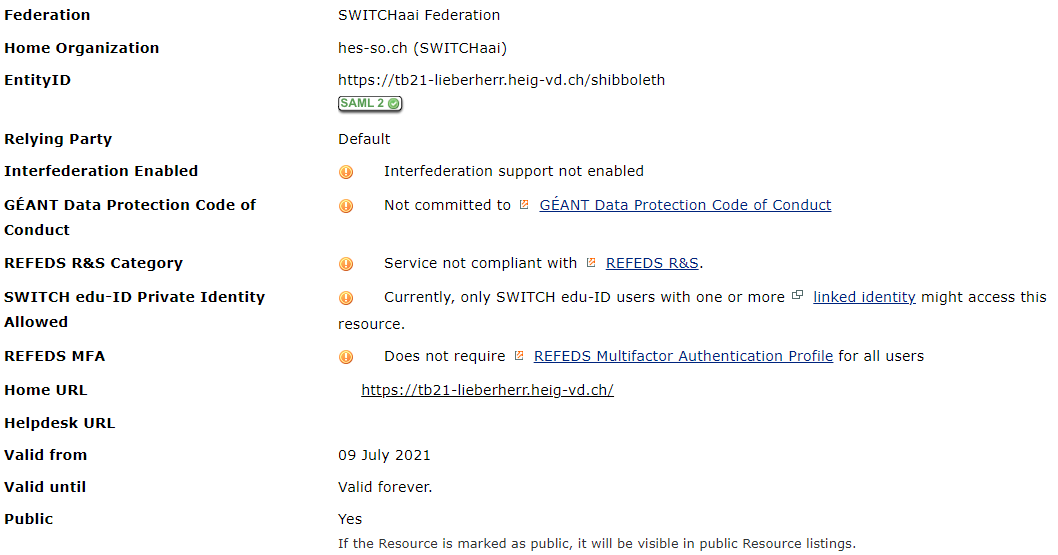
\includegraphics[width=14cm]{registry1.PNG}
  \caption{Aperçu de la ressource}
\end{figure}

\begin{figure}[h]
  \centering
  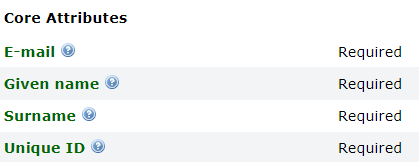
\includegraphics[height=3cm]{registry2.PNG}
  \caption{Attributs à disposition}
\end{figure}

Pour ce projet, l'organisation est la HES-SO (c'est eux qui possèdent l'identité des utilisateurs) et le service peut avoir accès à l'adresse email, au nom complet et à un identifiant unique des utilisateurs. La fiche complète est disponible à \href{https://rr.aai.switch.ch/view_resource.php?resource=11600}{cette adresse}.

Après ça, il faut ajouter des lignes dans le fichier de configuration "/etc/apache2/sites-enabled/000-default-le-ssl.conf" du serveur Apache. Ce fichier de configuration est expliqué au prochain chapitre, mais pour l'instant, il faut se contenter du code suivant :

\begin{figure}[h]
  \begin{minted}[breaklines]{html}
  <Location /Shibboleth.sso>
    SetHandler shib
  </Location>
  <Location />
    AuthType Shibboleth
    ShibRequestSetting requireSession false
    Require shibboleth
  </Location>
  \end{minted}
  \caption{code à ajouter dans le fichier de configuration}
  \label{code:Location}
\end{figure}

\newpage
La directive sous "<Location /Shibboleth.sso>" indique que les routes qui commencent par "/Shibboleth.sso" sont gérées par Shibboleth.
Celles sous "<Location />" indiquent que pour toutes les autres routes, c'est le service Shibboleth qui est utilisé pour l'authentification. Si "requireSession" vaut "true", ces routes sont verrouillées et si un utilisateur sans session valide tente d'y accéder, il est directement redirigé vers le service de découverte.

Il faut le laisser à "false" car ce n'est pas à ce niveau qu'on veut protéger l'accès au site : c'est à un étage plus bas, au niveau du code backend que celà doit avoir lieu.
Le schéma suivant illustre la situation :

\figi{protected_routes1.xml}{12cm}{Cheminement des routes web}

On y voit le cheminement des routes web. La route protégée est celle qui permet d'accéder à la SPA. Les routes qui commencent par "/Shibboleth.sso" sont automatiquement interceptées par Apache et gérées par Shibboleth. Pour qu'elles soient interceptées, il faut ajouter une directive dans le fichier ".htaccess" du dossier backend.

Ce fichier sert à imposer des directives dynamiques au serveur Apache, dynamiques dans le sens qu'il n'y a pas besoin de modifier les fichiers ".conf" et de redémarrer le serveur pour appliquer les changements. Les directives supplémentaires sont généralement propres projet backend, et peuvent simplement être modifiées sans nécessiter de redémarrage.
Laravel possède déjà ce fichier rempli par défaut, et il faut tout simplement ajouter une ligne juste en dessous de la ligne "RewriteCond \%{REQUEST\_FILENAME} !-f".

Les "RewriteCond" sont les conditions à respecter pour qu'un "RewriteRule" soit effectué. La réécriture des routes est très importante dans notre cas car elle permet de toujours passer par "index.php". Ce fichier est le point d'entrée de tout le site, et il est nécessaire de passer par cet endroit pour que les bonnes pages soient servies.

\newpage
Avec la nouvelle condition ajoutée, le premier noeud du schéma \ref{protected_routes1.xml} est créé : les routes qui commencent par "/Shibboleth.sso" ne sont pas transmises au backend. Au lieu de ça, c'est le service Shibboleth qui les reçoit et qui s'en occupe.

\begin{figure}[h]
  \begin{minted}[breaklines]{python}
  # Send Requests To Front Controller...
  RewriteCond %{REQUEST_FILENAME} !-d
  RewriteCond %{REQUEST_FILENAME} !-f
  RewriteCond %{REQUEST_URI} !^(/Shibboleth.sso) #à ajouter
  RewriteRule ^ index.php [L]
  \end{minted}
  \caption{aperçu du fichier ".htaccess"}
\end{figure}

Les autres routes sont donc gérées par le backend Laravel. À ce niveau, la route "/welcome" retourne la page d'accueil et toutes les autres sont gérées par la SPA. Au niveau de la SPA, c'est le routeur Vue qui s'occupe d'afficher les pages et de gérer les pages inexistantes.
Pour gérer le second noeud, celui de la couche backend, c'est simplement le code dans le fichier "web.php" qui s'en occupe.

Il reste encore une dernière étape pour que Laravel puisse gérer l'authentification avec Shibboleth. Pour cela, il faut installer le paquet "laravel-shibboleth" et suivre la procédure indiquée sur la \href{https://github.com/uabookstores/laravel-shibboleth}{page Github} du paquet.

Un nouveau fichier de configuration est créé sous "config/shibboleth.php". Il faut s'assurer que les valeurs suivantes soient appliquées :

\begin{figure}[h]
  \begin{minted}[breaklines]{javascript}
  'idp_login' => '/Shibboleth.sso/Login', //route de login
  'idp_logout' => '/Shibboleth.sso/Logout', //route de logout
  'authenticated' => '/', //route pour les utilisateurs authentifiés

  'entitlement' => 'uniqueID',

  'user' => [ //mapping des attributs mis à disposition par le IdentityProvider aux attributs du modèle Eloquent "User"
    'email' => 'mail',
    'name' => 'givenName',
    'surname' => 'surname',
  ],

  'add_new_users' => true, //les nouveaux utilisateurs doivent être ajoutés dans la base de données
  \end{minted}
  \caption{aperçu du fichier "shibboleth.php"}
\end{figure}

Quand un nouvel utilisateur est créé, son champ "password" dans la base de données est rempli avec la valeur "shibboleth", pour indiquer qu'il dépend du "Identity provider". Le mot de passe n'est en aucun cas utilisé pour authentifier un utilisateur. Les champs "email", "name" et "surname" sont automatiquement remplis avec les attributs fournis par le fournisseur d'identités.

\newpage
Il faut encore apporter un petit changement dans le fichier "config/auth.php" :

\begin{figure}[h]
  \begin{minted}[breaklines]{javascript}
  'providers' => [
    'users' => [
      'driver' => 'shibboleth', //il faut dire que Shibboleth s'occupe de l'authentification
      'model' => App\Models\User::class,
    ],
  ],
  \end{minted}
  \caption{aperçu du fichier "auth.php"}
\end{figure}

Il ne reste qu'une dernière étape pour que tout le système d'authentification fonctionne. Dans Laravel, quand un utilisateur veut accéder à une route protégée et qu'il n'est pas authentifié, la fonction "redirectTo()" située dans le fichier "app/Http/Middleware/Authenticate.php" est invoquée. Cette fonction doit retourner une route, est c'est par conséquent la route "/welcome" qui doit être retournée. Ainsi, quand l'utilisateur non authentifié veut accéder à une route protégée, il est toujours redirigé sur la page d'accueil.

Sur la page d'accueil, le lien vers le service de découverte redirige sur la route "/shibboleth-login". Cette route est automatiquement créée par la paquet, ainsi que la route "/shibboleth-logout". Ces routes sont gérées par Shibboleth et servent, comme leur nom l'indique, à se connecter et à se déconnecter de son compte.
Pour se déconnecter, il faut accéder à la route "/user/logout" de l'API. La fonction associée redirige vers la route "shibboleth-logout".

Au final, le site principal est accessible uniquement aux utilisateurs authentifiés. Il faut noter que si l'utilisateur se déconnecte, il n'est plus authentifié par Laravel et est envoyé sur la page d'accueil, mais sa session Shibboleth persiste tant qu'il ne ferme pas son navigateur. Il peut tenter d'accéder à nouveau au site, mais il n'aura cette fois pas besoin d'entrer ses identifiants.

\figi{shibboleth2.xml}{12cm}{Accès à une route protégée}

\newpage
\chapter{Déploiement}
Le déploiement du site nécessite d'utiliser un serveur HTTP qui tourne en permanance, afin de servir les pages et de répondre aux requêtes entrantes. Mais dans le cadre de ce projet, il faut aussi faire tourner un serveur websocket et un "Queue worker", qui sert à effectuer les travaux différés de manière asynchrone (emails).

Une machine virtuelle de l'école est utilisée à cet effet, avec comme système d'exploitation la version 20.04 d'Ubuntu. Il est possible de s'y connecter à distance via le protocole SSH. Le site est disponible à l'adresse \href{https://tb21-lieberherr.heig-vd.ch}{https://tb21-lieberherr.heig-vd.ch}.

\section{Code source}
Le code source se trouve sur Github. Il existe deux repos pour l'ensemble du projet : un pour le frontend et l'autre pour le backend.
Le repo du frontend se trouve à \href{https://github.com/TristanLieberherr/piaf}{cette page}, dans le repo "piaf". Puisqu'il s'agit du fork du site de base, il n'est pas publiquement visible.
La version du dernier commit est la 5ecb65d.

Le repo du backend se trouve à \href{https://github.com/TristanLieberherr/fablab-website}{cette page}, dans le repo "fablab-website". Ce repo est accessible et visible de tous. Il contient déjà la version compliée du frontend. La version du dernier commit est la 2280990.

Pour intégrer la SPA du frontend dans le code du backend, il faut d'abord compiler le projet. Lors de la compilation, les pages et composants Vue sont traduits en HTML, CSS et JavaScript.
Une fois terminé, le dossier "dist" est rempli avec deux fichiers et un dossier :
\begin{itemize}
  \item Le dossier "assets", qui contient les images, les logos, et le code JS et CSS.
  \item Le fichier "favicon.ico", qui est l'icône qui apparait dans le navigateur.
  \item Le fichier "index.html", qui contient la page HTML de lancement.
\end{itemize}
\bigskip

Ces trois éléments du dossier "dist" doivent ensuite être déposés dans le dossier "public" du backend. Il faut aussi impérativement copier le contenu de "index.html" pour le mettre dans "resources/views/app.blade.php".

\newpage
\section{Serveur Apache et certifical SSL}
Les détails concernant la configuration du serveur Apache se trouvent dans cette section. Le serveur Apache est un serveur HTTP. Son but est de répondre aux requêtes HTTP qui lui sont envoyées. C'est donc un processus qui tourne nuit et jour, et qui fait appel au code du backend pour répondre à ces requêtes. Apache s'occupe plus spécifiquement des requêtes web et API. Le serveur websocket est une autre entité qui sera abordé dans une autre section.

J'ai suivi \href{https://www.digitalocean.com/community/tutorials/how-to-secure-apache-with-let-s-encrypt-on-ubuntu-20-04}{ce tutoriel} pour l'obtention du certificat et de la sécurisation du serveur, ainsi que \href{https://www.digitalocean.com/community/tutorials/how-to-set-up-apache-virtual-hosts-on-ubuntu-18-04}{ce tutoriel} pour l'installation basique du serveur.
Il faut tout d'abord cloner le repo "fablab-website" qui contient le code du backend.

Ensuite, il faut installer Apache 2 et Certbot. Certbot est un exécutable qui automatise l'obtention d'un certifical SSL auprès de l'autorité de certification "Let's Encrypt". L'avantage est qu'en passant par eux, le certificat est gratuit. Ce certificat est nécessaire pour pouvoir utiliser le protocole sécurisé HTTPS.

Avant de lancer Certbot, il faut déjà ajouter quelques lignes dans le fichier de configuration de l'hôte virtuel sous "/etc/apache2/sites-available/000-default-le-ssl.conf". Un hôte virtuel permet à la machine de pouvoir gérer plusieurs serveurs virtuels en même temps, par exemple si plusieurs sites sont hébergés sur la même machine. Dans le cas de ce projet, il n'y en a qu'un seul.
Il faut ajouter les lignes ServerAdmin, DocumentRoot et ServerName, ainsi que configurer ce qui se trouve dans la balise "<Directory /var/www/fablab-website>". Par la suite, il faudra y ajouter quelques lignes pour tenir compte du certificat SSL.

\begin{figure}[h]
  \begin{minted}[breaklines]{html}
  <IfModule mod_ssl.c>
  <VirtualHost *:443> #le virtual host écoute sur le port 443
    ServerAdmin tristan.lieberherr@heig-vd.ch #email de l'admin
    DocumentRoot /var/www/fablab-website/public #chemin vers le dossier "public"
    ServerName tb21-lieberherr.heig-vd.ch #nom du serveur
    <Directory /var/www/fablab-website>
    Options Indexes FollowSymLinks
    AllowOverride All #pour pouvoir utiliser le .htaccess
    Require all granted #accepter toutes les requêtes
    Allow from all
    </Directory>
    <Location /Shibboleth.sso>
    SetHandler shib
    </Location>
    <Location />
    AuthType Shibboleth
    ShibRequestSetting requireSession false
    Require shibboleth
    </Location>
    ErrorLog ${APACHE_LOG_DIR}/error.log
    CustomLog ${APACHE_LOG_DIR}/access.log combined
  </VirtualHost>
  </IfModule>
  \end{minted}
  \caption{Aperçu du fichier "000-default-le-ssl.conf"}
\end{figure}

Avec cette première configuration, il est temps d'utiliser Certbot pour l'obtention du certificat. Le programme va demander quelques interactions textuelles et une fois terminé, le certificat est disponible et il se trouve dans le répertoire "/etc/letsencrypt/live/tb21-lieberherr.heig-vd.ch".

\newpage
Il est à présent nécessaire de l'inclure dans le fichier de configuration.

\begin{figure}[h]
  \begin{minted}[breaklines]{html}
    ...
    </Location>
    ErrorLog ${APACHE_LOG_DIR}/error.log
    CustomLog ${APACHE_LOG_DIR}/access.log combined
    #ajouter les trois lignes suivantes
    SSLCertificateFile /etc/letsencrypt/live/tb21-lieberherr.heig-vd.ch/fullchain.pem #chemin vers la chaine complète
    SSLCertificateKeyFile /etc/letsencrypt/live/tb21-lieberherr.heig-vd.ch/privkey.pem #chemin vers la clé privée
    Include /etc/letsencrypt/options-ssl-apache.conf
  </VirtualHost>
  </IfModule>
  \end{minted}
  \caption{Ajout du certificat au fichier de configuration}
\end{figure}

Les certificats délivrés par Let's Encrypt ne durent que 90 jours, il faut donc un système pour les renouveler automatiquement. Heureusement, Certbot s'en occupe déjà. Il n'y a donc pas besoin de se soucier de la validité du certificat, qui est vérifiée deux fois par jour par le programme. Il faut juste s'assurer qu'il fonctionne en faisant un essai à blanc.

Pour finir, il faut reprendre le fichier ".htaccess" et y ajouter une dernière directive pour limiter la taille des requêtes à 5 MB, limite fixée pour l'envoi des fichiers. Il suffit simplement d'ajouter une ligne vers la fin du fichier :

\begin{figure}[h]
  \begin{minted}[breaklines]{python}
    ...
    RewriteRule ^ index.php [L]

    php_value upload_max_filesize 5M #à ajouter
    </IfModule>
  \end{minted}
  \caption{Ajout de la limite d'upload}
\end{figure}

Désormais, les requêtes HTTP passent en HTTPS, et si le navigateur Chrome est utilisé, un icône de verrou indique que la navigation est sécurisée.

\newpage
\section{Processus supervisés}
Pour que le système soit totalement fonctionnel, il a besoin de deux autres services : le serveur websocket et le "Queue worker", qui est le precessus qui s'occupe d'effectuer les travaux différés de manière asynchrone, pour les emails. Pour qu'ils puissent tourner en permanence et qu'ils soient capables de se relancer en cas d'erreur, il faut faire appel à un logiciel de contrôle de processus.
Ce logiciel s'appelle Supervisor.

Une fois l'installation terminée, il faut créer deux nouveaux fichiers qui correspondent aux deux services qu'il faut gérer. Les fichiers s'appellent "laravel-queue.conf" et "laravel-websocket.conf", situés sous "/etc/supervisor/conf.d". Ces fichiers contiennent la configuration de chaque service.

\begin{figure}[h]
  \begin{minted}[breaklines]{python}
  [program:laravel-queue]
  process_name=%(program_name)s_%(process_num)02d #nom du processus
  command=php /var/www/fablab-website/artisan queue:work #commande à effectuer
  user=root #utilisateur en tant que qui exécuter la commande
  autostart=true #permet de démarrer tout seul
  autorestart=true #permet de redémarrer en cas de fermeture
  numprocs=1 #nombre de processus. 1 seul suffit pour les deux services
  \end{minted}
  \caption{laravel-queue.conf}
\end{figure}

\begin{figure}[h]
  \begin{minted}[breaklines]{python}
  [program:laravel-websocket]
  process_name=%(program_name)s_%(process_num)02d
  command=php /var/www/fablab-website/artisan websockets:serve
  user=root
  autostart=true
  autorestart=true
  numprocs=1
  \end{minted}
  \caption{laravel-websocket.conf}
\end{figure}

Tant que Supervisor est en service, il va s'occuper de ces processus. En cas de souci, ils sont redémarrés automatiquement. Si nécessaire, il est possible de créer plusieurs processus par service, mais ce n'est pas le cas pour ce projet.

\newpage
\chapter{Conclusion}





\chapter{Introduction}
L'introduction est une section requise dans un rapport technique. Introduisez votre travail, l'idée de départ et les objectifs attendus. Un lecteur qui découvrirait votre projet au travers de cette introduction devrait ainsi être capable d'en comprendre le cadre, l'idée générale et les aboutissants du projet.

\section{Contexte}
Cette section \underline{n'est pas obligatoire}, mais elle est souvent présente dans un rapport technique pour compléter l'introduction et définir le contexte du travail \cad le cadre formel dans lequel le travail est mené.

%%if
\section{Citations et bibliographie}
Citer vos sources est essentiel. Avec \texttt{biblatex} vous pouvez facilement citer des articles, des livres ou des sites internet. Toutes les citations dans le texte seront automatiquement regroupées en fin de document dans la section \guillemotleft Bibliographie\guillemotright. Par exemple, citons un article d'Einstein \cite{einstein} ou le livre de Dirac \cite{dirac}.

Parfois il peut être utile d'utiliser un gestionnaire de bibliographie. La communauté académique recommande l'outil \href{https://www.zotero.org/}{Zotero} qui permet de gérer une bibliothèque numérique d'ouvrages et de références numériques. Il permet également de générer une bibliographie compatible avec \LaTeX.

\section{Exemple d'équation}
L'une des principales forces de \LaTeX est la saisie d'équations. L'équation \ref{eq:1}, citée à titre d'exemple, représente la transformation de phase d'une lentille biconvexe. Pour rédiger une équation \LaTeX vous pouvez utiliser des outils en ligne tels que \href{https://www.latex4technics.com/}{latex4technics}.

\begin{equation} \label{eq:1}
  \begin{split}
    L(x,y) &= \exp\left( - i\frac{{2\pi }}{\lambda }\left( {n\Delta \varphi (x,y) + \Delta {\varphi _0} - \Delta \varphi (x,y)} \right)\right)\\
    &= {\exp\left({i\frac{{2\pi }}{\lambda }\Delta {\varphi _0}}\right)}{\exp\left({ - i\frac{{2\pi }}{{\lambda f}}({x^2} + {y^2})}\right)}
  \end{split}
\end{equation}

\section{Exemples de diagrammes}

Les diagrammes de flux peuvent être réalisés en utilisant l'outil \href{https://app.diagrams.net/}{draw.io}. Une exportation en \texttt{.xml} (non compressé) permet de garder les sources de la figure. Le rendu en \texttt{.pdf} sera réalisé à la volée à la compilation. L'intérêt est double : n'avoir qu'une source de vérité \cad pas d'image intermédiaire à stocker, et réduire la quantité d'information stockée.

Puisque la source est au format XML, les textes sont accessibles au correcteur orthographique et il vous est rendu possible les modifier sans avoir à éditer l'image. La figure \ref{euclide.xml} en est un exemple.


\figi{euclide.xml}{9cm}{Algorithme d'Euclide}

Notons qu'il est inutile d'insérer des images coloriées là où la couleur n'offre aucune valeur ajoutée ; évitez également les ombrages et autres effets de style. Enfin, préférez toujours des représentations vectorielles là où c'est possible.

Voici un autre type de diagramme utile (figure \ref{sequence.xml}), celui d'une séquence UML.

\figi{sequence.xml}{8cm}{Diagramme de séquence}

\section{Exemple de figure}

Pour présenter des résultats d'expérience, vous pouvez soit dessiner des graphiques manuellement en utilisant des outils de dessin vectoriel comme Inkscape ou Adobe Illustrator comme illustré à la figure \ref{plot.svg} ou alors, vous pouvez utiliser Python ou Matlab. Avec ce dernier choix, vous pouvez générer vos figures à la volée : le code source \ref{python} permet de générer la figure \ref{bode.py}.

\fig{plot.svg}{Exemple de graphique plan}

\begin{listing}[h]
  \inputminted[breaklines]{php}{assets/figures/php.php}
  \caption{Génération d'un diagramme de Bode \label{python}}
\end{listing}


\figi{bode.py}{12cm}{Diagramme de Bode généré à la volée}

\clearpage

\subsection{Schémas électroniques}
Vous pouvez également utiliser TikZ pour créer vos propres schémas électriques et électroniques comme l'exemple \ref{circuit}.

\begin{figure}[h]
  \begin{center}
    \begin{circuitikz}
      \draw
      (0,0) to [short, *-] (6,0)
      to [V, l_=$\mathrm{j}{\omega}_m \underline{\phi}^s_R$] (6,2)
      to [R, l_=$R_R$] (6,4)
      to [short, i_=$\underline{i}^s_R$] (5,4)
      (0,0) to [open, v^>=$\underline{u}^s_s$] (0,4)
      to [short, *- ,i=$\underline{i}^s_s$] (1,4)
      to [R, l=$R_s$] (3,4)
      to [L, l=$L_{\sigma}$] (5,4)
      to [short, i_=$\underline{i}^s_M$] (5,3)
      to [L, l_=$L_M$] (5,0);
    \end{circuitikz}
    \caption{Circuit électrique \label{circuit}}
  \end{center}
\end{figure}

\subsection{Dessins techniques}
L'intégration de dessins mécaniques est préférée en vue filaire. SolidWorks conserve la représentation vectorielle à l'exportation. À partir du PDF généré, l'image peut être isolée et sauvegardée en format SVG.

\begin{figure}[!ht]
  \begin{center}
    \includegraphics[width=10cm]{\assetsdir/assembly.svg.\graphicsExt}
  \end{center}
  \caption[Assemblage mécanique]{\label{assembly}Réducteur cycloïdale de puissance comportant 6. l'axe de sortie, 14. le roulement de sortie, 1. le corps du réducteur en aluminium, 3 et 5. les disques cycloïdaux et 2. les goupilles de prise... D'autres informations liées à la figure elle-même peuvent aussi figurer dans la légende}
\end{figure}

Notez ici que la légende est particulièrement longue. Celle que vous retrouverez dans la table figures est plus courte. La commande \mintinline{latex}{\caption[courte]{longue}} permet de saisir une légende courte, pour la table des figures et longue pour le corps du document.

La figure \ref{assembly} est un dessin technique épuré qui permet de décrire un phénomène ou un fonctionnement important dans le rapport technique. Les mises en plan détaillées seront quant à elles disponibles en annexes.

\clearpage
\section{Tableaux}

Concernant les tableaux, restez simple et minimaliste, n'ajoutez des séparateurs que là ou c'est nécessaire pour améliorer la lisibilité. Une liste de quelques cantons suisses est donnée à titre d'exemple dans la table \ref{cantons}.

\begin{table}[h]
  \begin{center}
    \caption{Liste des cantons \label{cantons}}
    \begin{tabular}{c|l|r}
      Abréviation & Nom du canton & Depuis                  \\ \hline
      ZH          & Zürich        & \ordinalnum{1} mai 1351 \\
      BE          & Berne         & 6 mars 1353             \\
      FR          & Fribourg      & 22 décembre 1481        \\
      VD          & Vaud          & 19 février 1815         \\
      VS          & Valais        & 4 août 1815             \\
      NE          & Neuchâtel     & 19 mai 1815             \\
      GE          & Genève        & 19 mai 1815
    \end{tabular}
  \end{center}
\end{table}

Si vous devez donner une spécification technique, n'oubliez pas de mentionner les valeurs minimales, maximales et nominales sans omettre l'unité de mesure. Notez que les séparateurs verticaux sont souvent critiqués pour réduire la lisibilité mais parfois ils sont utiles. Utilisez-les avec parcimonie.

\begin{table}[h]
  \begin{center}
    \caption{Exigences techniques \label{specification}}
    \begin{tabularx}{\textwidth}{cXcccc}
      No. & Exigence                                                                   & Min. & Nom. & Max. & Unité                           \\ \toprule
      E1  & Tension d'alimentation                                                     & 12   & 24   & 48   & \si{\volt}                      \\ \midrule
      E2  & Fréquence                                                                  & 50   &      & 60   & \si{\hertz}                     \\ \midrule
      E3  & Concentration                                                              &      & 300  & 1200 & \si{\nano\gram\per\milli\litre} \\ \midrule
      E4  & \multicolumn{5}{l}{Doit pouvoir être stoppé à l'aide d'un arrêt d'urgence}
    \end{tabularx}
  \end{center}
\end{table}

L'exemple de la table \ref{specification}, assigne pour chaque exigence un numéro unique. Cette table est \textbf{normative}, chaque élément doit pouvoir être référencé par un identifiant unique (cf. T\ref{specification}-E3). Dans le cas ou cet identifiant est utilisé en dehors de ce document, la version du document devra être renseignée.

\section{Index}
\LaTeX~ permet d'indexer les mots \index{mots} importants. Il suffit de placer les termes importants d'un paragraphe dans la commande \texttt{\textbackslash index\{terme\}} et ils apparaitront automatiquement à la fin de ce rapport dans l'index du document.

\index{Napoléon}

Imaginons que dans cette section nous parlions du cheval blanc \index{cheval blanc} de Napoléon. Il se pourrait que le lecteur recherche ce passage dans la version imprimée du rapport. Avec l'index, rien de plus facile. Allez jeter un oeil à la page \pageref{index}.

\section{Notes de bas de page}

\maraja{Je suis une marginale, et je suis utile pour résumé un paragraphe en quelques mots.} Parfois, il est plus élégant d'annoter une définition en utilisant une note de bas de page \footnote{La note en bas de page (ou note de bas de page) est une forme littéraire, consistant en une ou plusieurs lignes ne figurant pas dans le texte.}. Alternativement il est possible d'annoter un paragraphe avec une note marginale.

\section{Glossaire et acronymes}

La \Gls{heig-vd} membre de la \Gls{hes-so} propose ce modèle de document. Le format \LaTeX est particulièrement adapté pour les documents qui contiennent des expressions mathématiques. Pour plus de détail sur l'utilisation d'un glossaire, se référer à \url{https://www.overleaf.com/learn/latex/Glossaries}. Tient donc, ci-dessus nous utilisons deux acronymes. Les trouverez-vous dans le glossaire en page \pageref{glossaire} ?

\section{Unités de mesure}

Lorsque vous mentionnez des quantités, utilisez les unités du système international. \LaTeX~et le paquet \textsf{siunitx} permet la saisie de quantités. La commande suivante permet d'afficher \SI{42.12}{\kilo\gram\metre\per\square\second}.\par

\mintinline{latex}{\SI{42.12}{\kilo\gram\metre\per\square\second}}\par
%%fi

%%if
Bien que non nécessaire dans un rapport de Bachelor, la discussion finale d'un projet résume les résultats obtenus et dresse une conclusion objective du projet. Un manager de société est souvent amené à lire de nombreux rapport, il ne s'intéresse généralement qu'à l'introduction au contexte de l'étude et à sa conclusion.

Il est de coutume de signer la conclusion...
%%fi

\vfil
\hspace{8cm}\makeatletter\@author\makeatother\par
\hspace{8cm}\begin{minipage}{5cm}
  %%if
  % Place pour signature numérique
  \printsignature
  %%fi
\end{minipage}
\clearpage

\appendix
\appendixpage
\addappheadtotoc

%%if
\chapter{Première annexe}
Cette annexe contient quelques fichiers sources détaillants l'utilisation de l'API.

\section{Code source backend}

\begin{figure}[h]
  \inputminted[breaklines]{javascript}{assets/code/2014_10_12_000000_create_users_table.php}
  \caption{2014\_10\_12\_000000\_create\_users\_table.php}
\end{figure}

\begin{figure}[h]
  \inputminted[breaklines]{javascript}{assets/code/2019_08_19_000000_create_failed_jobs_table.php}
  \caption{2019\_08\_19\_000000\_create\_failed\_jobs\_table.php}
\end{figure}

\begin{figure}[h]
  \inputminted[breaklines]{javascript}{assets/code/2021_04_01_075350_create_jobs_table.php}
  \caption{2021\_04\_01\_075350\_create\_jobs\_table.php}
\end{figure}

\begin{figure}[h]
  \inputminted[breaklines]{javascript}{assets/code/2021_04_23_123136_create_files_table.php}
  \caption{2021\_04\_23\_123136\_create\_files\_table.php}
\end{figure}

\begin{figure}[h]
  \inputminted[breaklines]{javascript}{assets/code/2021_04_28_140349_create_timeline_events_table.php}
  \caption{2021\_04\_28\_140349\_create\_timeline\_events\_table.php}
\end{figure}

\begin{figure}[h]
  \inputminted[breaklines]{javascript}{assets/code/2021_05_26_122557_create_jobsQueue_table.php}
  \caption{2021\_05\_26\_122557\_create\_jobsQueue_table.php}
\end{figure}

\begin{figure}[h]
  \inputminted[breaklines]{javascript}{assets/code/2021_05_30_144810_create_messages_table.php}
  \caption{2021\_05\_30\_144810\_create\_messages\_table.php}
\end{figure}

\begin{figure}[h]
  \inputminted[breaklines]{javascript}{assets/code/api.php}
  \caption{api.php}
\end{figure}

\begin{figure}[h]
  \inputminted[breaklines]{javascript}{assets/code/web.php}
  \caption{web.php}
\end{figure}

\begin{figure}[h]
  \inputminted[breaklines]{javascript}{assets/code/FileController.php}
  \caption{FileController.php}
\end{figure}

\begin{figure}[h]
  \inputminted[breaklines]{javascript}{assets/code/JobController.php}
  \caption{JobController.php}
\end{figure}

\begin{figure}[h]
  \inputminted[breaklines]{javascript}{assets/code/MessageController.php}
  \caption{MessageController.php}
\end{figure}

\begin{figure}[h]
  \inputminted[breaklines]{javascript}{assets/code/UserController.php}
  \caption{UserController.php}
\end{figure}

\section{Code source frontend}

\begin{figure}[h]
  \inputminted[breaklines]{javascript}{assets/code/index.js}
  \caption{index.js}
\end{figure}

Les annexes n'ont pas un contenu \underline{normatif} mais \underline{descriptif}. Tout contenu annexé ne doit pas être nécessaire à la bonne compréhension du travail.

Les annexes contiennent généralement :

\begin{itemize}
  \item les dessins mécaniques (mises en plan);
  \item les schémas électriques détaillés;
  \item des photographies du projet;
  \item des scripts et des extraits de code source;
  \item des documents techniques \pex \emph{datasheet};
  \item des développements mathématiques.
\end{itemize}
\section{Sous section}
\lipsum[1]
%%fi

\let\cleardoublepage\clearpage
\backmatter

\label{glossaire}
\printnoidxglossary
\printbibliography
\label{index}
\printindex

%%if
\clearpage
\Large\textbf{Colophon :}\par\normalsize
\thispagestyle{empty}
La qualité de cet ouvrage repose que le moteur \LaTeX. La mise en page et le format sont inspirés d'ouvrages scientifiques tels que le modèle de thèse de l'EPFL et celui des publications O'Reilly.

Les diagrammes et les illustrations sont édités depuis l'outil en ligne draw.io. Certaines illustrations ont été reprises dans Adobe Illustrator. Les représentations 3D sont exportées de SolidWorks et certains graphiques sont générés à la volée depuis un code source Python.

L'auteur fictive de ce document \emph{Maria Bernasconi} est un nom emprunté, par amusement, aux spécimens publiés par Postfinance.

Ce document a été compilé avec XeLaTeX.

La famille de police de caractères utilisée est \emph{Computed Modern} créée par Donald Knuth avec son logiciel METAFONT.
\vfil
Le Colophon est le dernier élément d'un document qui contient des notes de l'auteur concernant la mise en page et l'édition du document : il est parfaitement optionnel.
%%fi

\end{document}
